\chapter{THE LHC AND THE CMS EXPERIMENT}\label{Ch2}

European Organisation for Nuclear Research, best know as CERN, is established in 1954 by 12 European countries and is based at the Franco-Swiss border in northwest Geneva, Switzerland. Today, the organisation operates the largest particle physics laboratory in the world and has 23 member states \cite{CERN:2771424} and many others that make up more than 11 thousand researches and more than 70 countries around the globe. CERN's main activity is to provide the particle accelerators and needed infrastructure for high energy physics research. The organisation hosts the LHC Experiment which is the world's largest particle collider.

This chapter introduces the structure and operations of the LHC and the CMS Detector on which the simulated Monte Carlo event samples are based in this thesis.

\section{The Large Hadron Collider}

The Large Hadron Collider consists of a 27-kilometre ring tunnel where the beams of particles (protons or lead ions) are accelerated with the help of superconducting magnets along with a number of accelerating systems. It was built between 1998 and 2008 and it lies 175 metres beneath the surface with a total cost of the project expected to be of the order of 4.4\$ billion. The initial design of the LHC aimed at the centre-of-mass energy of $\sqrt{s}=14$ TeV with a nominal peak luminosity of $\mathcal{L} = 10^{34}cm^{-2}s^{-1}$ \cite{Baconnier:257706}. The LHC collides proton-proton beams as well as lead-lead (Pb - Pb), proton-lead (p - PB) and Xenon-Xenon (Xe - Xe) nuclei to study heavy-ion collisions. The \textbf{\emph{LHC accelerator complex}} consist of a series of accelerators and is used to accelerate protons before being injected in the LHC, which will be explained shortly.

\subsection{Operation of the LHC}

The success of the LHC required two decade-long international collaboration. The initial studies started in the early 1980s when the The Large Electron Positron Collider (LEP) at CERN was not even running. CERN Council approved the construction of the LHC in 1994 and a technical design report was published the next year. Starting from 1998, the construction of the LHC was completed in 2008 and it succeeded to accelerate proton beams the same year \cite{lhcfirstbeams}. The first accelerated proton beams had an energy of 450 GeV per beam and later on the collisions at $\sqrt{s}=2.14$ TeV with respect to Tevatron at 1.96 TeV and made the LHC the highest-energy collider ever built. In 2010, LHC increased the beam energy to 3.5 TeV which was a world record of man-made particle acceleration.

Data collection started in 2010 and finished in 2013; this time period is known as Run I of the LHC. The CMS Experiment collected about 45$pb^{-1}$, 6 $fb^{-1}$ and 23 $fb^{-1}$ data at $\sqrt{s}=7$ TeV in 2010, 2011 and 2012, respectively. The data collected at Run I has lead the discovery of the Higgs boson. LHC entered an upgrade stage called Long Shutdown 1 (LS1) for two years when Run I is finished in 2012. LHC was upgraded in LS1 in the way of achieving its design performances, and started its operation again in 2015 for a period of 3 years known as Run II but his time the beam energy was 6.5 TeV. The Run II is finished in 2018 with a data amounting to about 150 $fb^{-1}$ and LHC entered LS2 with a schedule to be in Run III in 2022 at $\sqrt{s}=14$ TeV. The LS3 is planned to be the update period where the LHC will have an unprecedented instantaneous luminosity corresponding to an integrated luminosity of 3000 to 4000 $fb^{-1}$ eventually, called the High-Luminosity LHC (HL-LHC) or Phase II. Both the LHC and the HL-LHC plans shown in \autoref{HLLHCplan}.

\begin{figure}[ht]
	\centering
	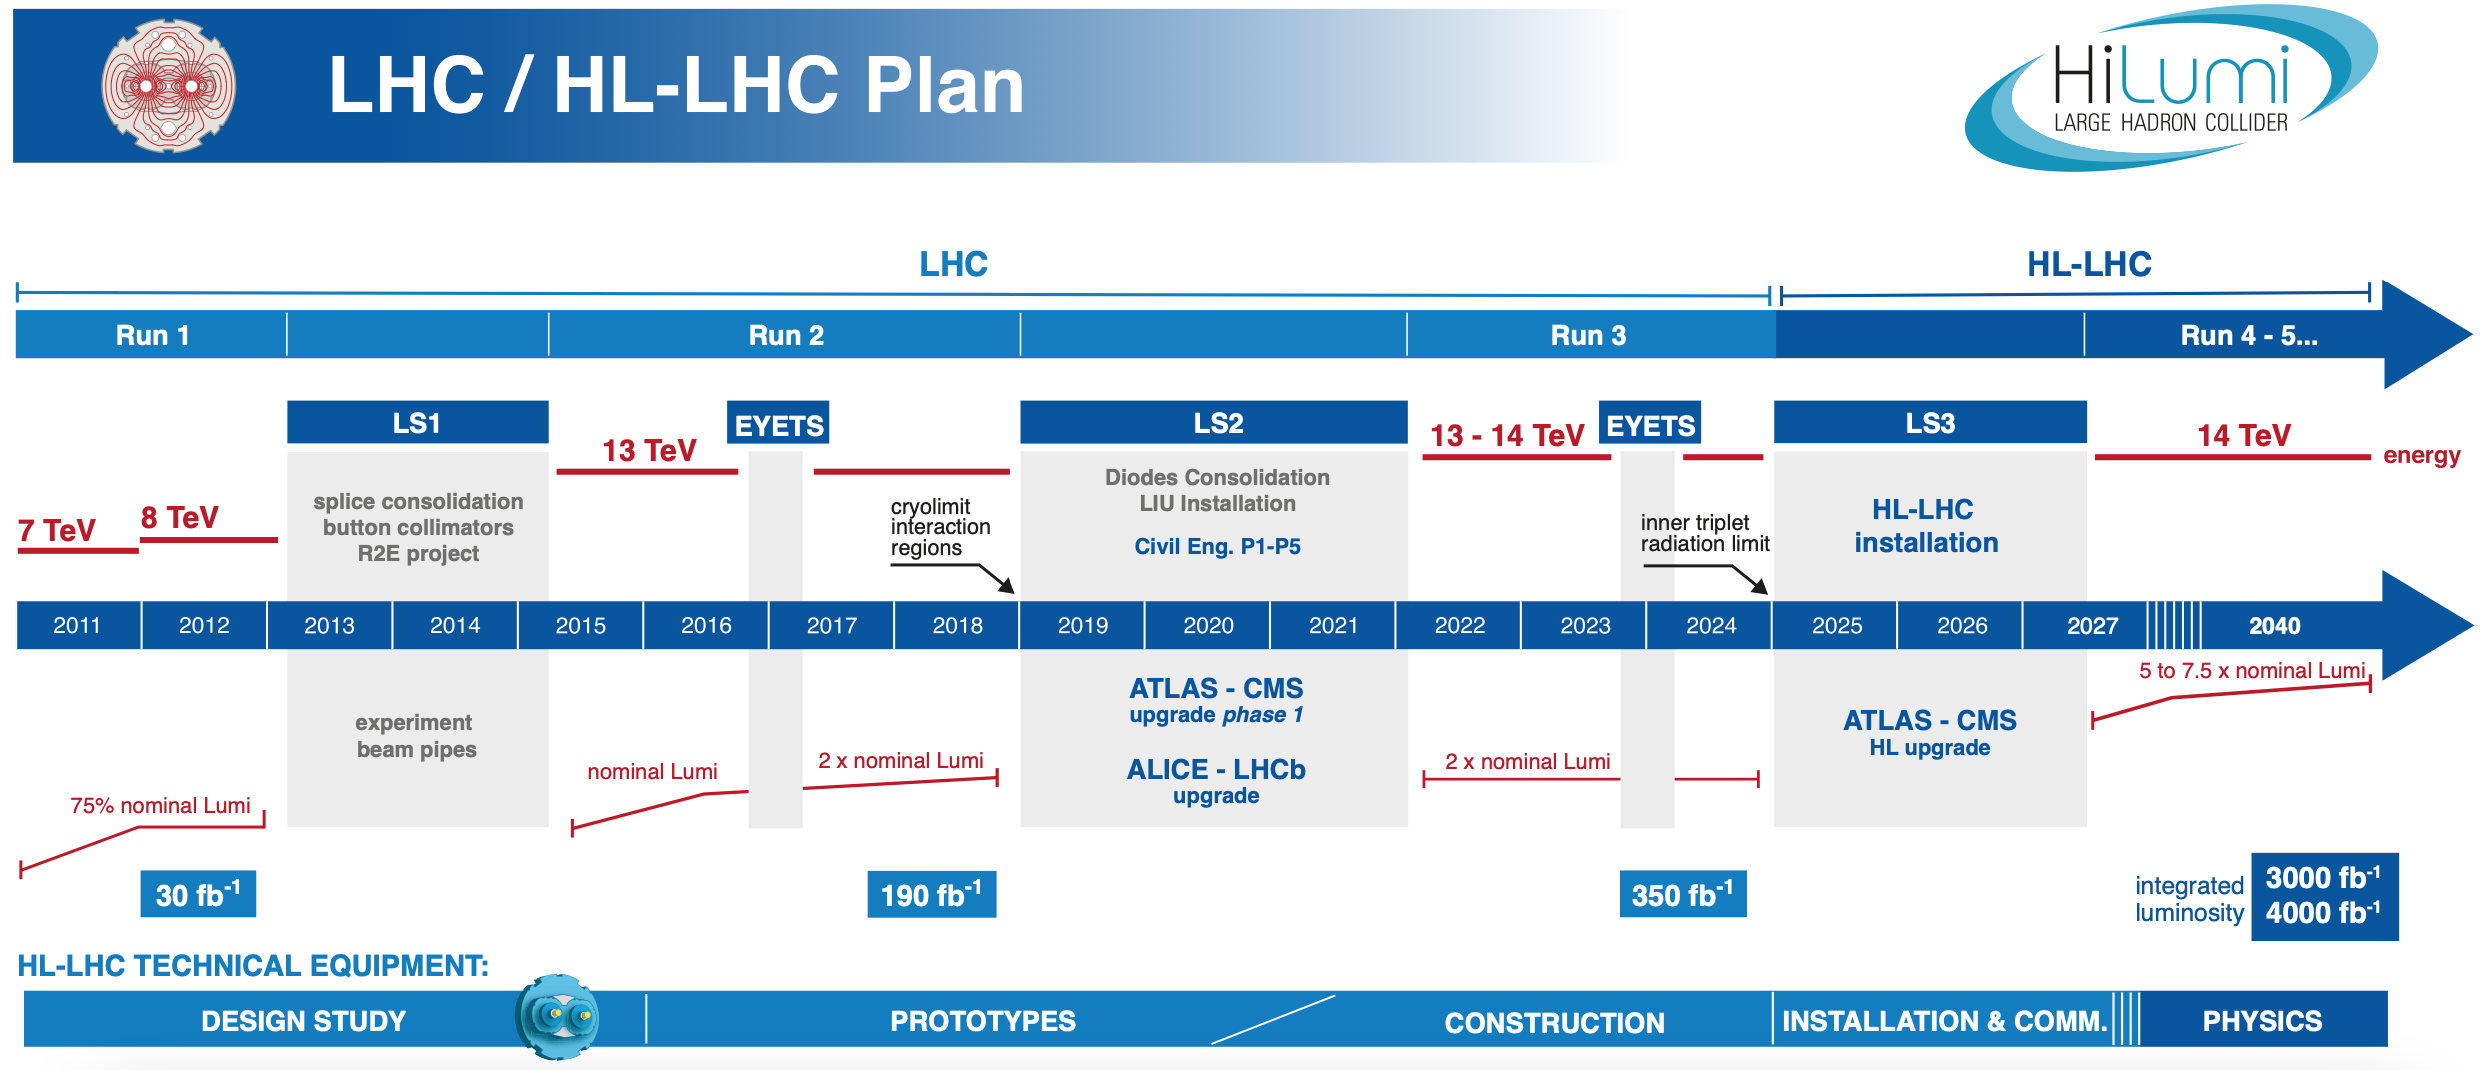
\includegraphics[width=\textwidth]{HLLHCplan.png}
	\vspace{2mm}
	\caption[A detailed schedule of LHC and HL-LHC showing the integrated luminosity and the beam energy corresponding to each period.]
	{A detailed schedule of LHC and HL-LHC showing the integrated luminosity and the beam energy corresponding to each period \cite{Apollinari:2284929}.}
	\label{HLLHCplan}
\end{figure}

The main scope of the HL-LHC is to increase the collision data which will allow physics searches to be more statistically abundant and be able to perform higher-precision measurements.

\subsection{The accelerator complex}

The accelerator tunnel of the LHC, which was previously used host LEP collider, has two parallel vacuum pipes where two counter-rotating beams are kept inside a magnetic field generated by superconducting niobium-titanium (NbTi) cables. The magnetic field generated to steer the beams are about 8 Tesla which is more than 100 000 times higher than the Earth2s magnetic field. This field is generated by  1232 dipole magnets each with a 14 metres of length and 35 tonnes of weight where 11 thousand Ampers of electric current flows. This acceleration system allow the beams to circulate with 7 TeV energy. The focusing of the beams in a narrow area is secured by 392 quadrupole magnets with 5 to 7 m lengths. In order to inject the beams in the collision points, special quadrupoles are positioned at each entrance to squeeze the beams in a narrower area. These superconducting magnets are cooled down to a temperature of 1.9 K by a cyrogenics cooling system supplied with 120 tonnes of Helium-4 fluid.

Before being injected into the LHC, the proton beams are pulled off from hydrogen gas and accelerated by a series of systems gradually increasing their energy, presented in \autoref{LHCacc}. Firstly, protons are accelerated to an energy of 50 MeV in the Linear Accelerator (LINAC2) then injected into the Proton Synchrotron Booster (PSB) where beams are re-accelerated to 1.4 GeV. These particles are sent to the Super Proton Synchrotron (SPS) to further accelerate them to 450 GeV energy. The final injection is made from the SPS to LHC's two beam pipes in the counter directions. The filling of the LHC by protons takes about 8 minutes, and 20 minutes for protons to be accelerated to 6.5 TeV of energy in bunches via Radio Frequency (RF) cavities operating. The injected beams circulate the LHC rings for many hours (12 hours) under normal operation. The bunches are spaced by 25 ns or 7.5 metres thus the bunch crossing rate is 40 MHz. Nominal number of protons per bunch is $12x10^{11}$ and the nominal number of bunches per beam is 2808 contributing to an inelastic collision event in the order of $10^9$ per second with about 20 collisions per bunch crossing.

\begin{figure}[ht]
	\centering
	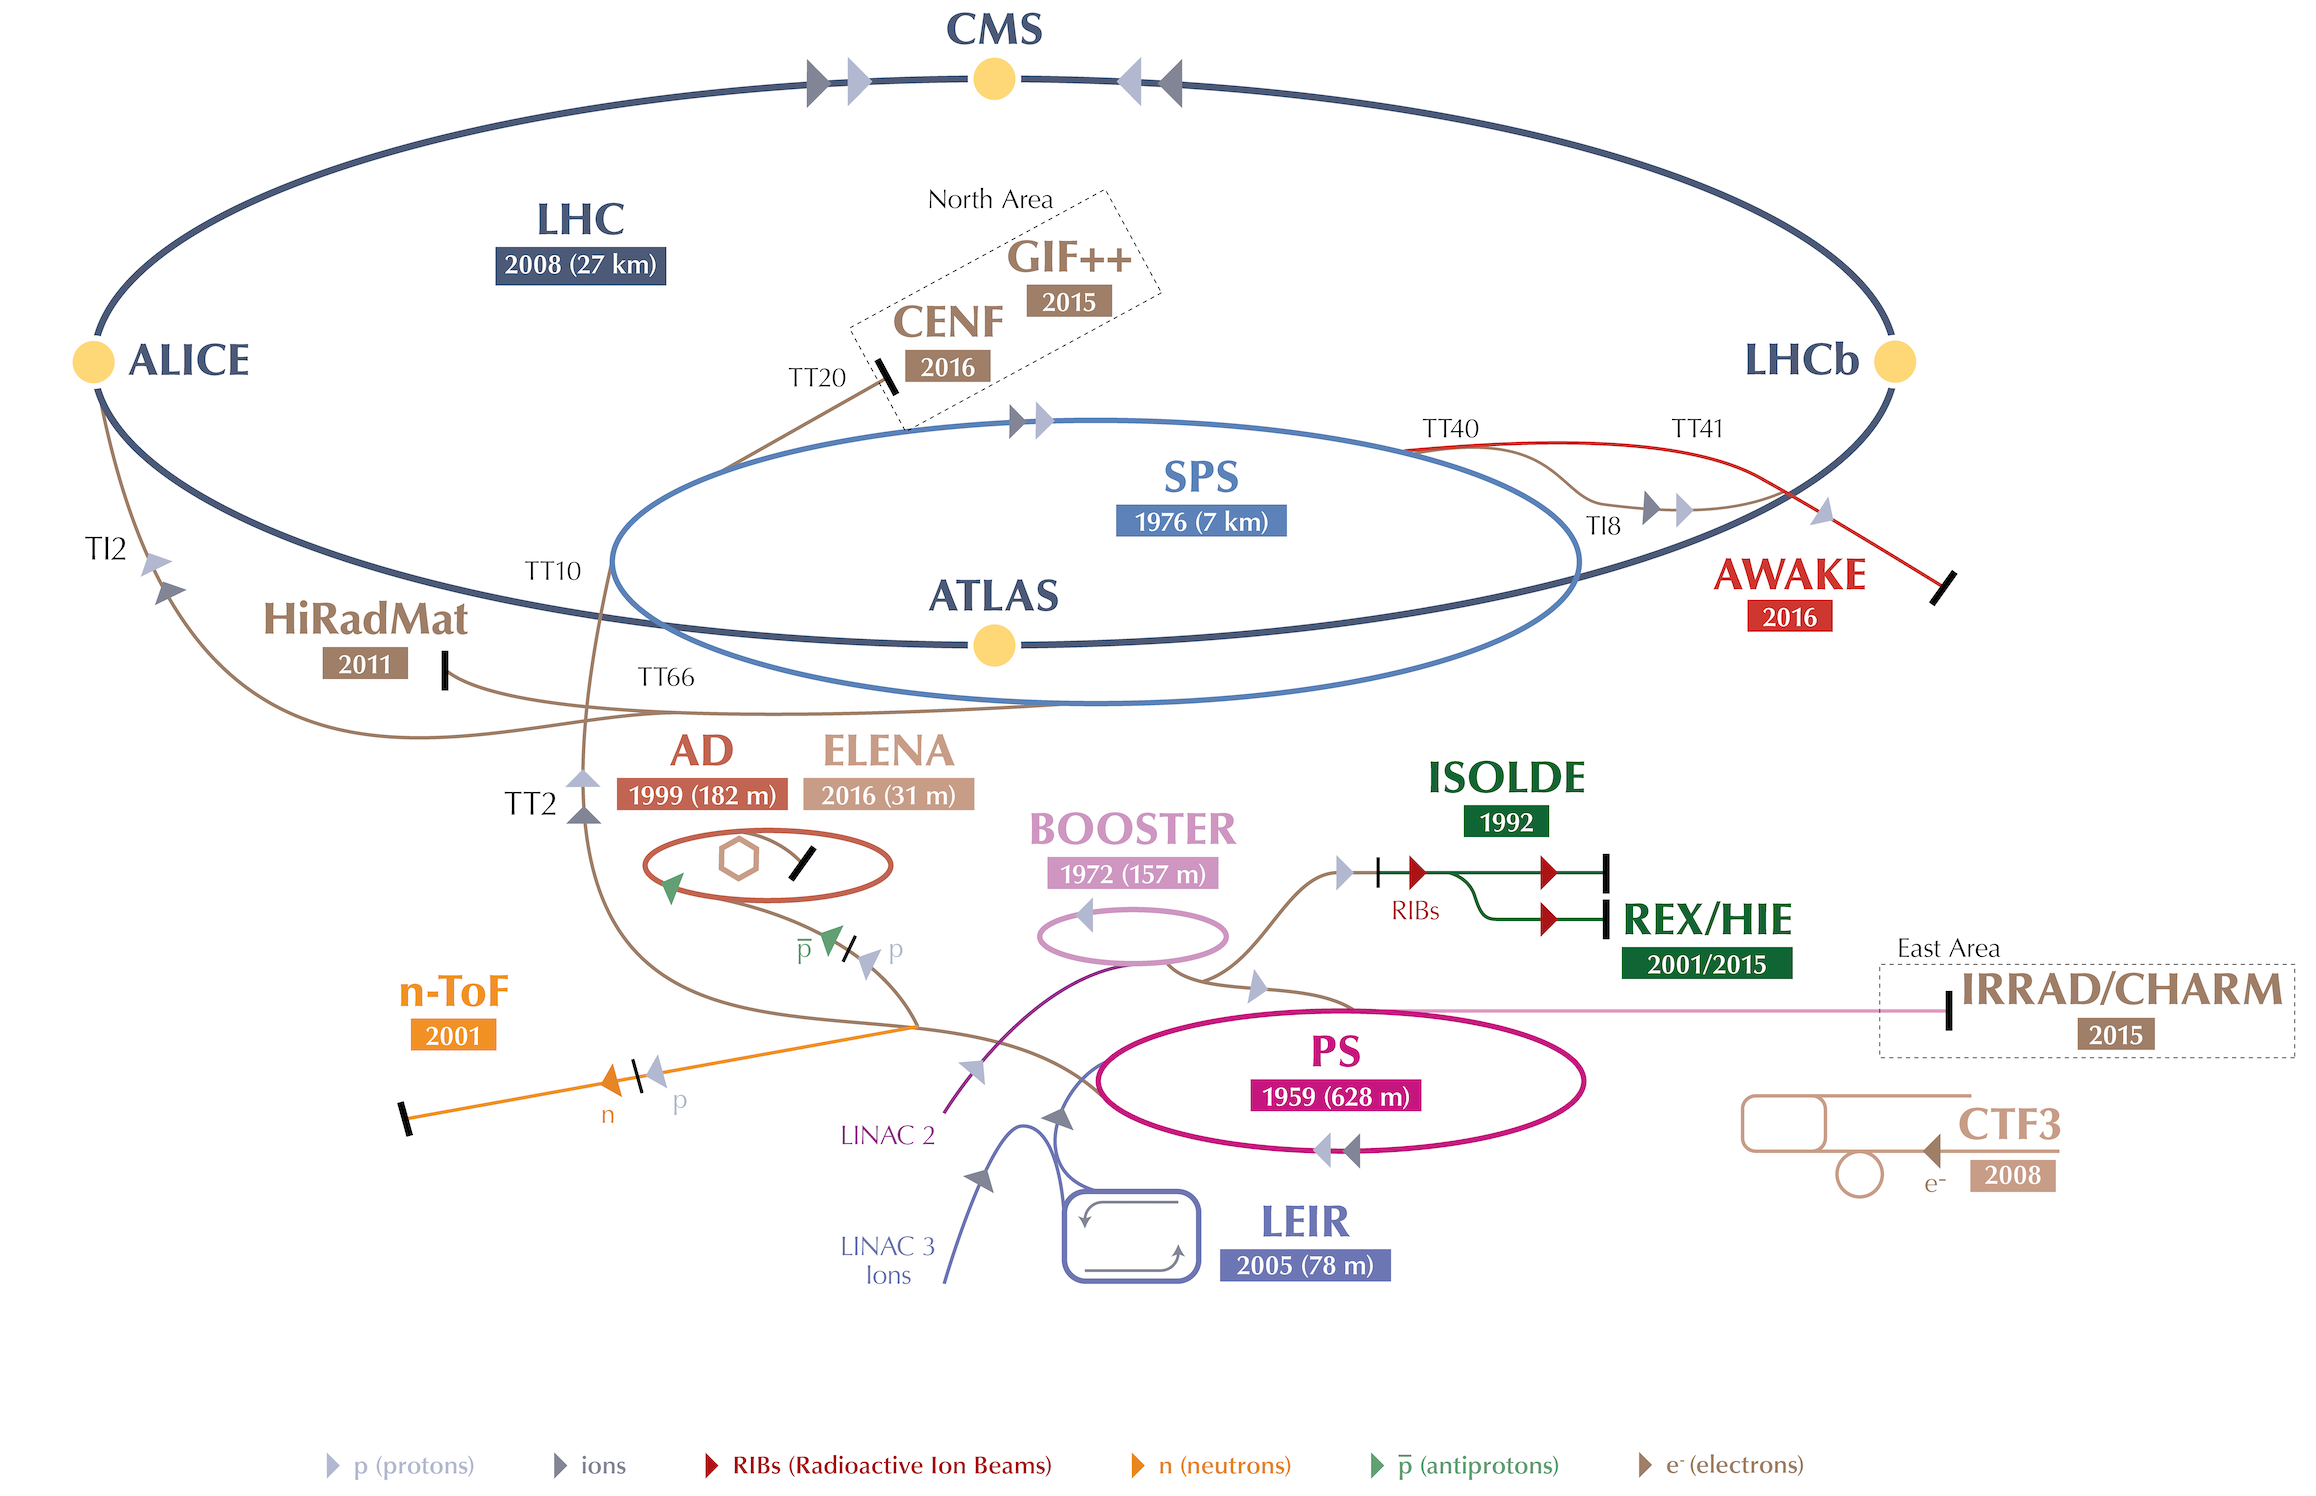
\includegraphics[width=\textwidth]{LHCacc.png}
	\vspace{2mm}
	\caption[The LHC accelerator complex. The acceleration of the protons start in the LINAC2 and ends in LHC through Booster, PS and SPS.]
	{The LHC accelerator complex. The acceleration of the protons start in the LINAC2 and ends in LHC through Booster, PS and SPS \cite{Mobs:2197559}.}
	\label{LHCacc}
\end{figure}

The accelerated beams of particles are collided inside one of the four detectors; ALICE, ATLAS, CMS and LHCb. The ATLAS and CMS Detectors are installed in opposite sides, at Point 1 and Point 5 of the LHC. These two detectors are designed as multi-purpose detectors that surround the collision points to detect any out-coming particle. They are described in detail in the references \cite{ATLAS2008, CMS2008}. ALICE Experiment is installed at Point 2 and its main purpose is to study heavy ion collisions and quark-gluon plasmas. Final of the four large experiments, LHCb, located at Point 8, is a forward one sided detector mainly aimed at measuring the charge conjugation and parity symmetry violation in Beauty baryons. The detailed description of the two detectors can be found in \cite{ALICE2008, LHCb2008}.

LHC host many other experiments; the LHCf \cite{LHCF2006} and TOTEM \cite{TOTEM2004} Experiments positioned at 100 meters away from the both sides of the ATLAS and CMS's collision points. These experiment study mainly the pp interactions and forward physics. Others are the MoEDAL\cite{moedal} Experiment which is dedicated to search for magnetic monopoles at the same experimental cavern with LHCb detector, and the FASER Experiment searching for lighter particles and studying neutrinos situated 480 metres away from the ATLAS's collision point.

\subsection{Design and specifications}

The \textbf{\emph{collision energy}} of the particles inside the detectors is one of the most important parameters at the LHC and is simply the sum of the energy of two colliding beams. When these collisions happen, independent types of interactions may happen between protons. The \textbf{\emph{soft interactions}} signify a small amount of transferred momentum which means the interacting protons barely came close to each other and escapes without decaying at all. The \textbf{\emph{hard interactions}} on the other hand, signify a high transferred momentum which causes the proton to decay. When two protons collide, a fraction of the energy ($s\prime$) contributes to the interaction since it is actually the partons of the protons that participate in the collision proportional to the fraction of energies ($x_1,\; x_2$) of each parton.
\be
\sqrt{s\prime} = \sqrt{x_1 x_2 s}
\ee
Another important parameter is the \textbf{\emph{instantaneous luminosity}} for the LHC apparatus. It is a description of the number of collisions per time and cross section. It is given by the following formula,
\be
L = \frac{N_b^2 n_b f_{rev} \gamma}{4 \pi \epsilon_n \beta}F \; ,
\ee
where $N_b$ is the number of particles in each bunches of $n_b$ bunches circulating in the accelerator ring with $f_{rev}$ frequency. The parameters $\gamma$, $\epsilon_n$, $\beta$ and the factor $F$ denotes the relativistic Lorentz factor; emittence and focal length describing the shape and focus of the beam, and geometrical reduction which depends on the angle between two beams, respectively. The luminosity lifetime $\tau$ on the other hand shows how luminosity decreases with time,
\be
L = L_0 e^{-t/\tau} \; ,
\ee
where $L_0$ is the peak luminosity at time zero.

The integrated luminosity, which is another important parameter, is given by $L = \int L dt$ and takes part in the total amount of collisions over time.
\be
N = L x \sigma
\ee
is the number of events produced for a particular physics process with the cross section $\sigma$. Thus, in order for a rare process to be observed in the detectors, maximising the luminosity is essential. In \autoref{SMcrosssections}, the cross sections as a function of $\sqrt{s}$ is shown. It is obvious that the Higgs processes are several orders of magnitude lower in production cross section than the dominant processes, however since the cross section increases with the increasing centre-pf-mass energy, it is necessary to increase also luminosity and $\sqrt{s}$ in order to achieve higher event rates. The integrated luminosity delivered to the CMS experiment since 2010 is shown in \autoref{CMSlumi}.
\begin{figure}[ht]
	\centering
	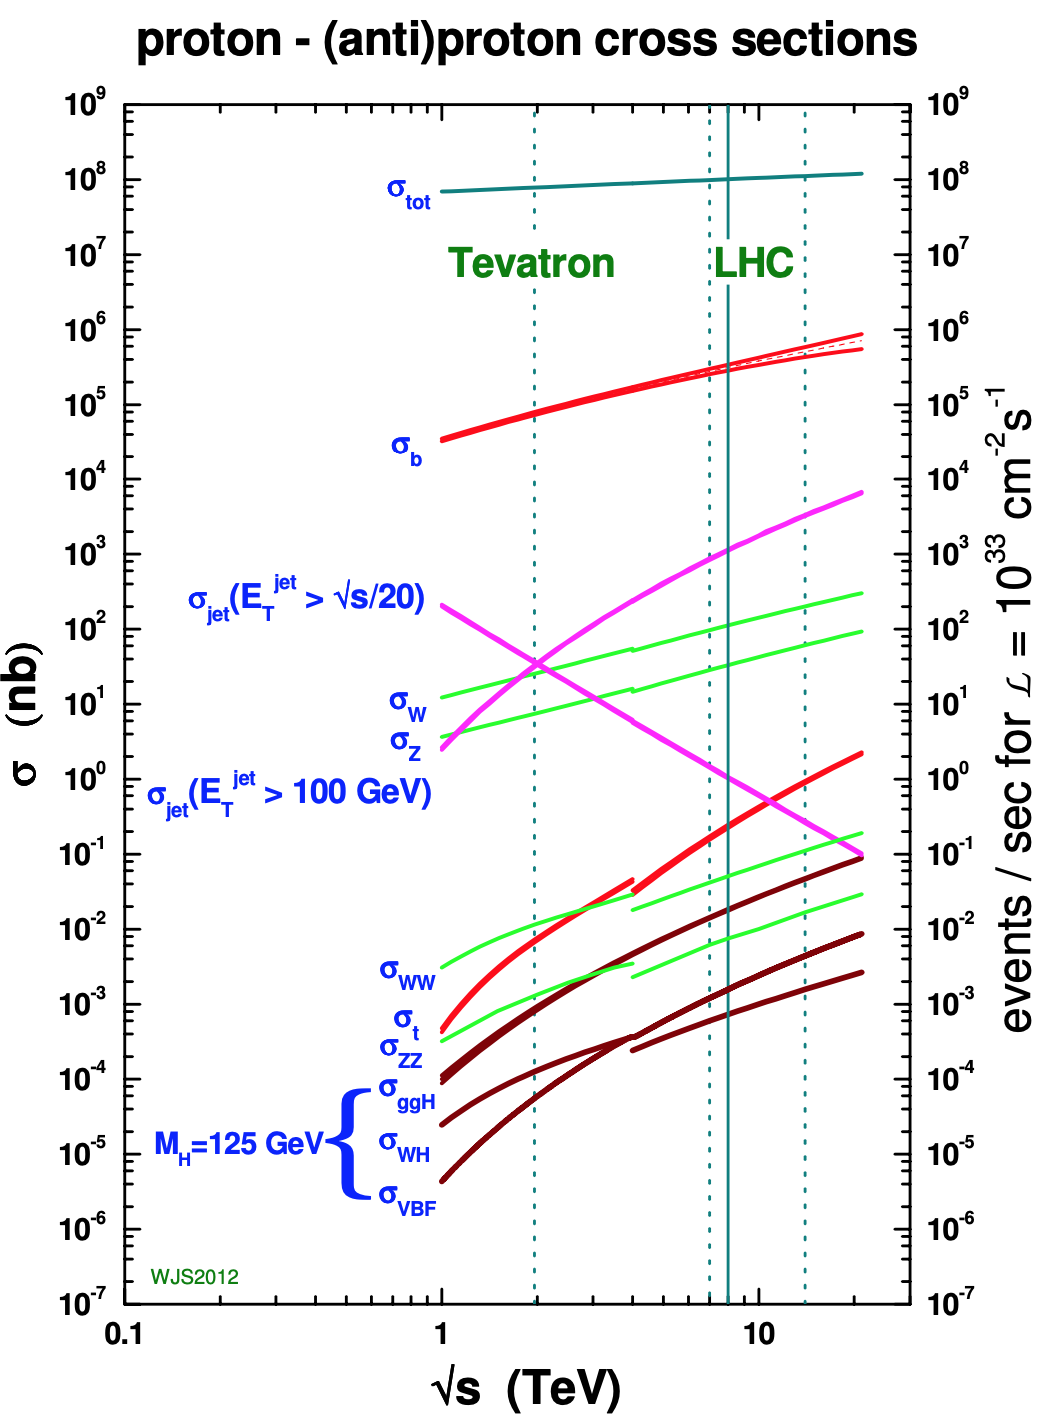
\includegraphics[scale=0.5]{stirling.png}
	\vspace{2mm}
	\caption[Cross sections of Standard Model processes as function of collider energy at pp collisions.]
	{Cross sections of Standard Model processes as function of collider energy at pp collisions\cite{stirling}.}
	\label{SMcrosssections}
\end{figure}

The large instantaneous luminosity of the LHC causes a disadvantage. Multiple pp collisions happen at each bunch crossing and many primary vertices are superimposed. Most of these parton interactions have relatively small centre-of-mass energy, hence they are not of much interest for the experiment, which is often called \textbf{\emph{in-time pileup (PU)}} interactions. Therefore, the detector needs to resolve these pileup interactions from the hard collisions. Besides, since the collisions take place at the heart of the CMS detector, it is inevitable that new particles reach the detector before the products of the previous bunch crossing escapes the detector. This type of pile up is called \textbf{\emph{out-of-time pileup}} interactions. In order to overcome these demanding conditions, highly granular and fast-response detectors are needed. Moreover, the detector needs to be resistant to radiation as well as be precise in energy measurements. The Compact Muon Solenoid, an appropriate detector designed to overcome these challenges, is explained in the next section.

\begin{figure}[ht]
	\centering
	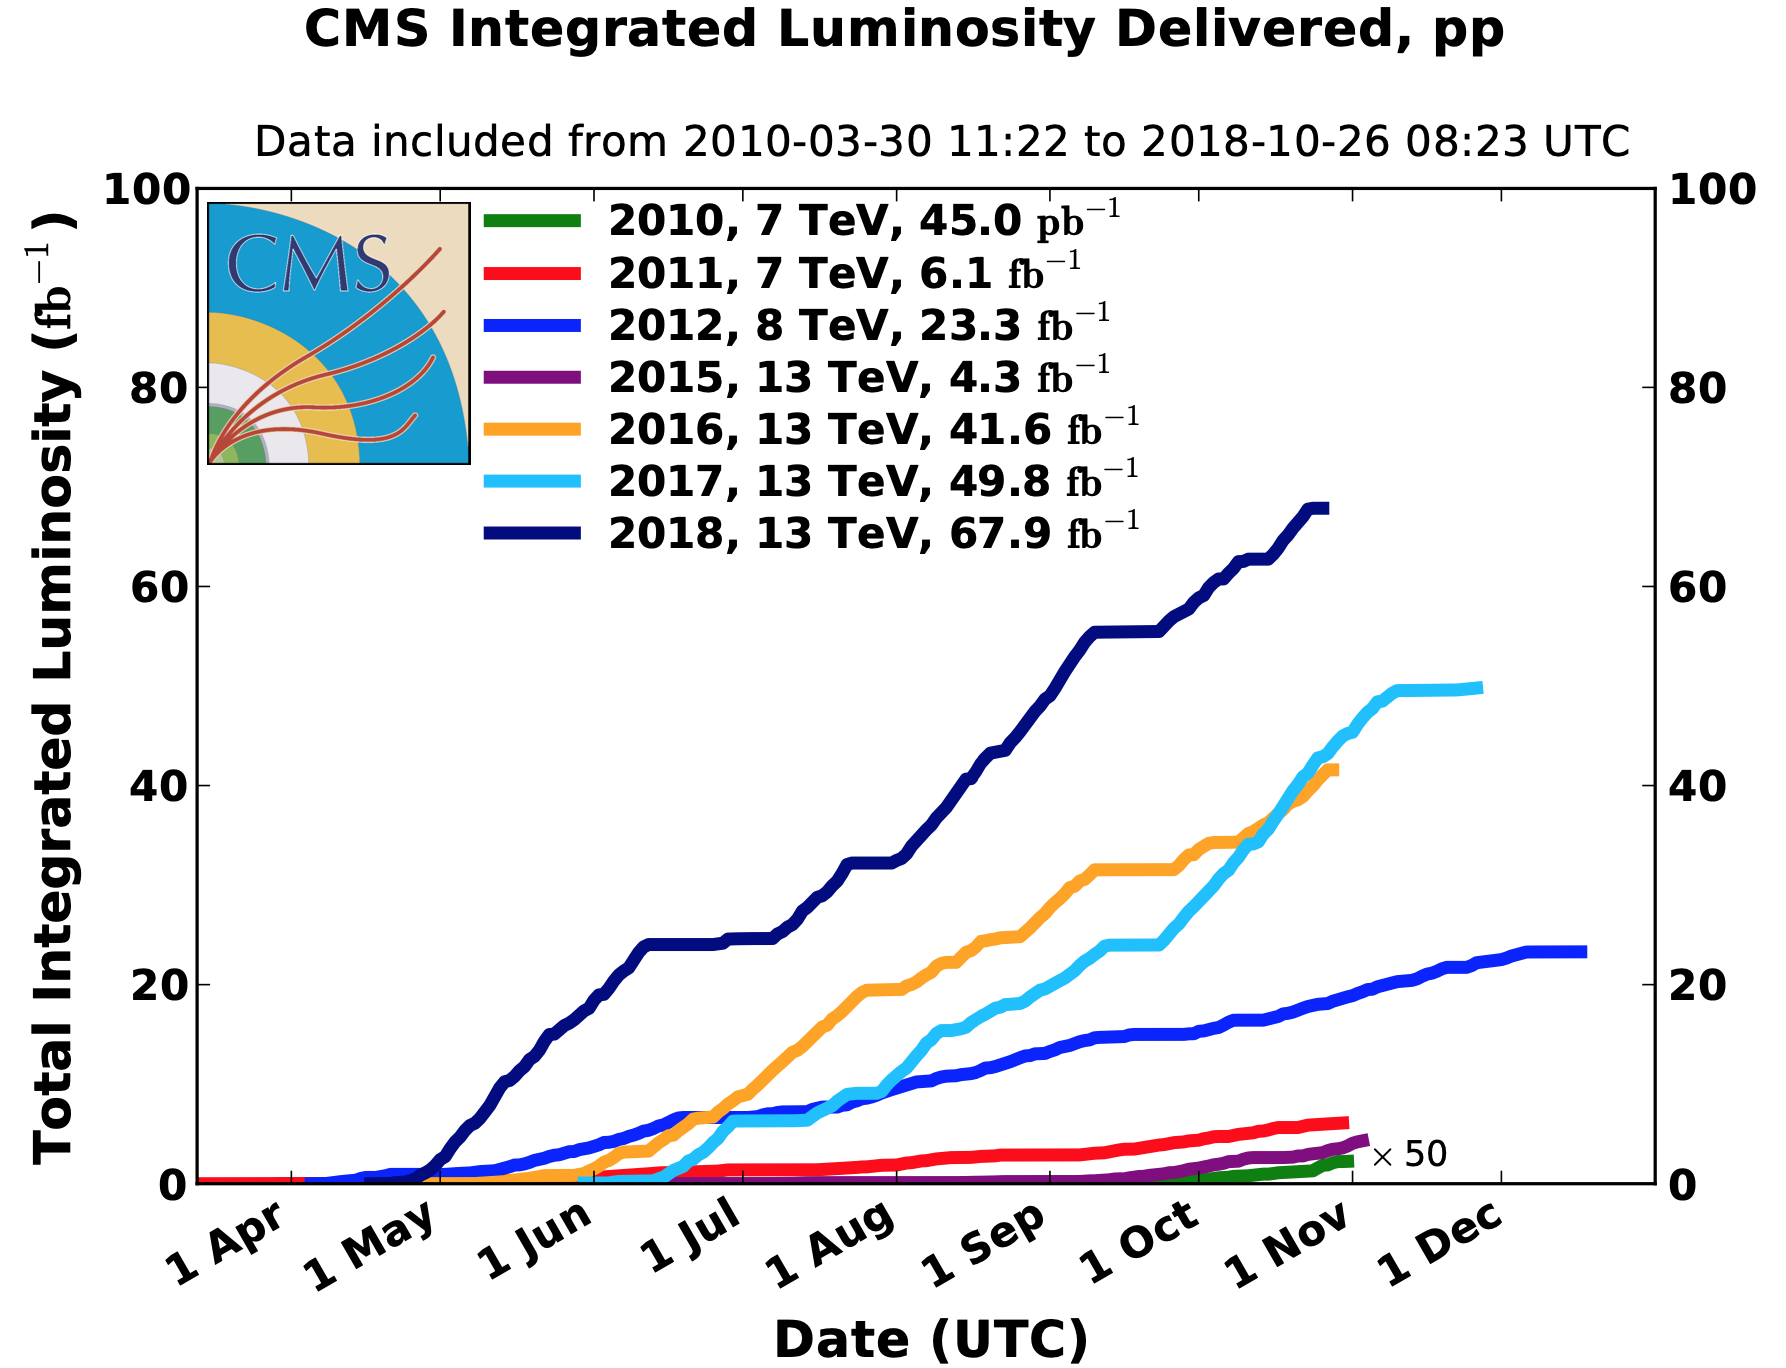
\includegraphics[scale=0.4]{CMSlumi.png}
	\vspace{2mm}
	\caption[Total integrated luminosity delivered by the LHC to the CMS detector for pp collisions at Run I-II.]
	{Total integrated luminosity delivered by the LHC to the CMS detector for pp collisions at Run I-II \cite{CMSlumi}.}
	\label{CMSlumi}
\end{figure}

\section{The Compact Muon Solenoid Experiment}

The CMS Collaboration, consisting of more than 4000 particle physicist, engineers, technicians and student from around 200 institutes and more than 40 countries, is a  particle physics community in search for the fundamental building blocks of our universe. The collaboration operates the CMS detector and collects data from the collision of the protons supplied by the LHC. It is one of the two multi-purpose detectors at the LHC facility, and has a broad physics program. Each term in its name means one of the detector's main features; \textbf{\emph{Compact}} signifies its small size for all the detector material it contains, \textbf{\emph{Muon}} emphasises the dedicated muon tracking system and \textbf{\emph{Solenoid}} underlines the most powerful solenoid magnet ever made.

\begin{figure}[ht]
	\centering
	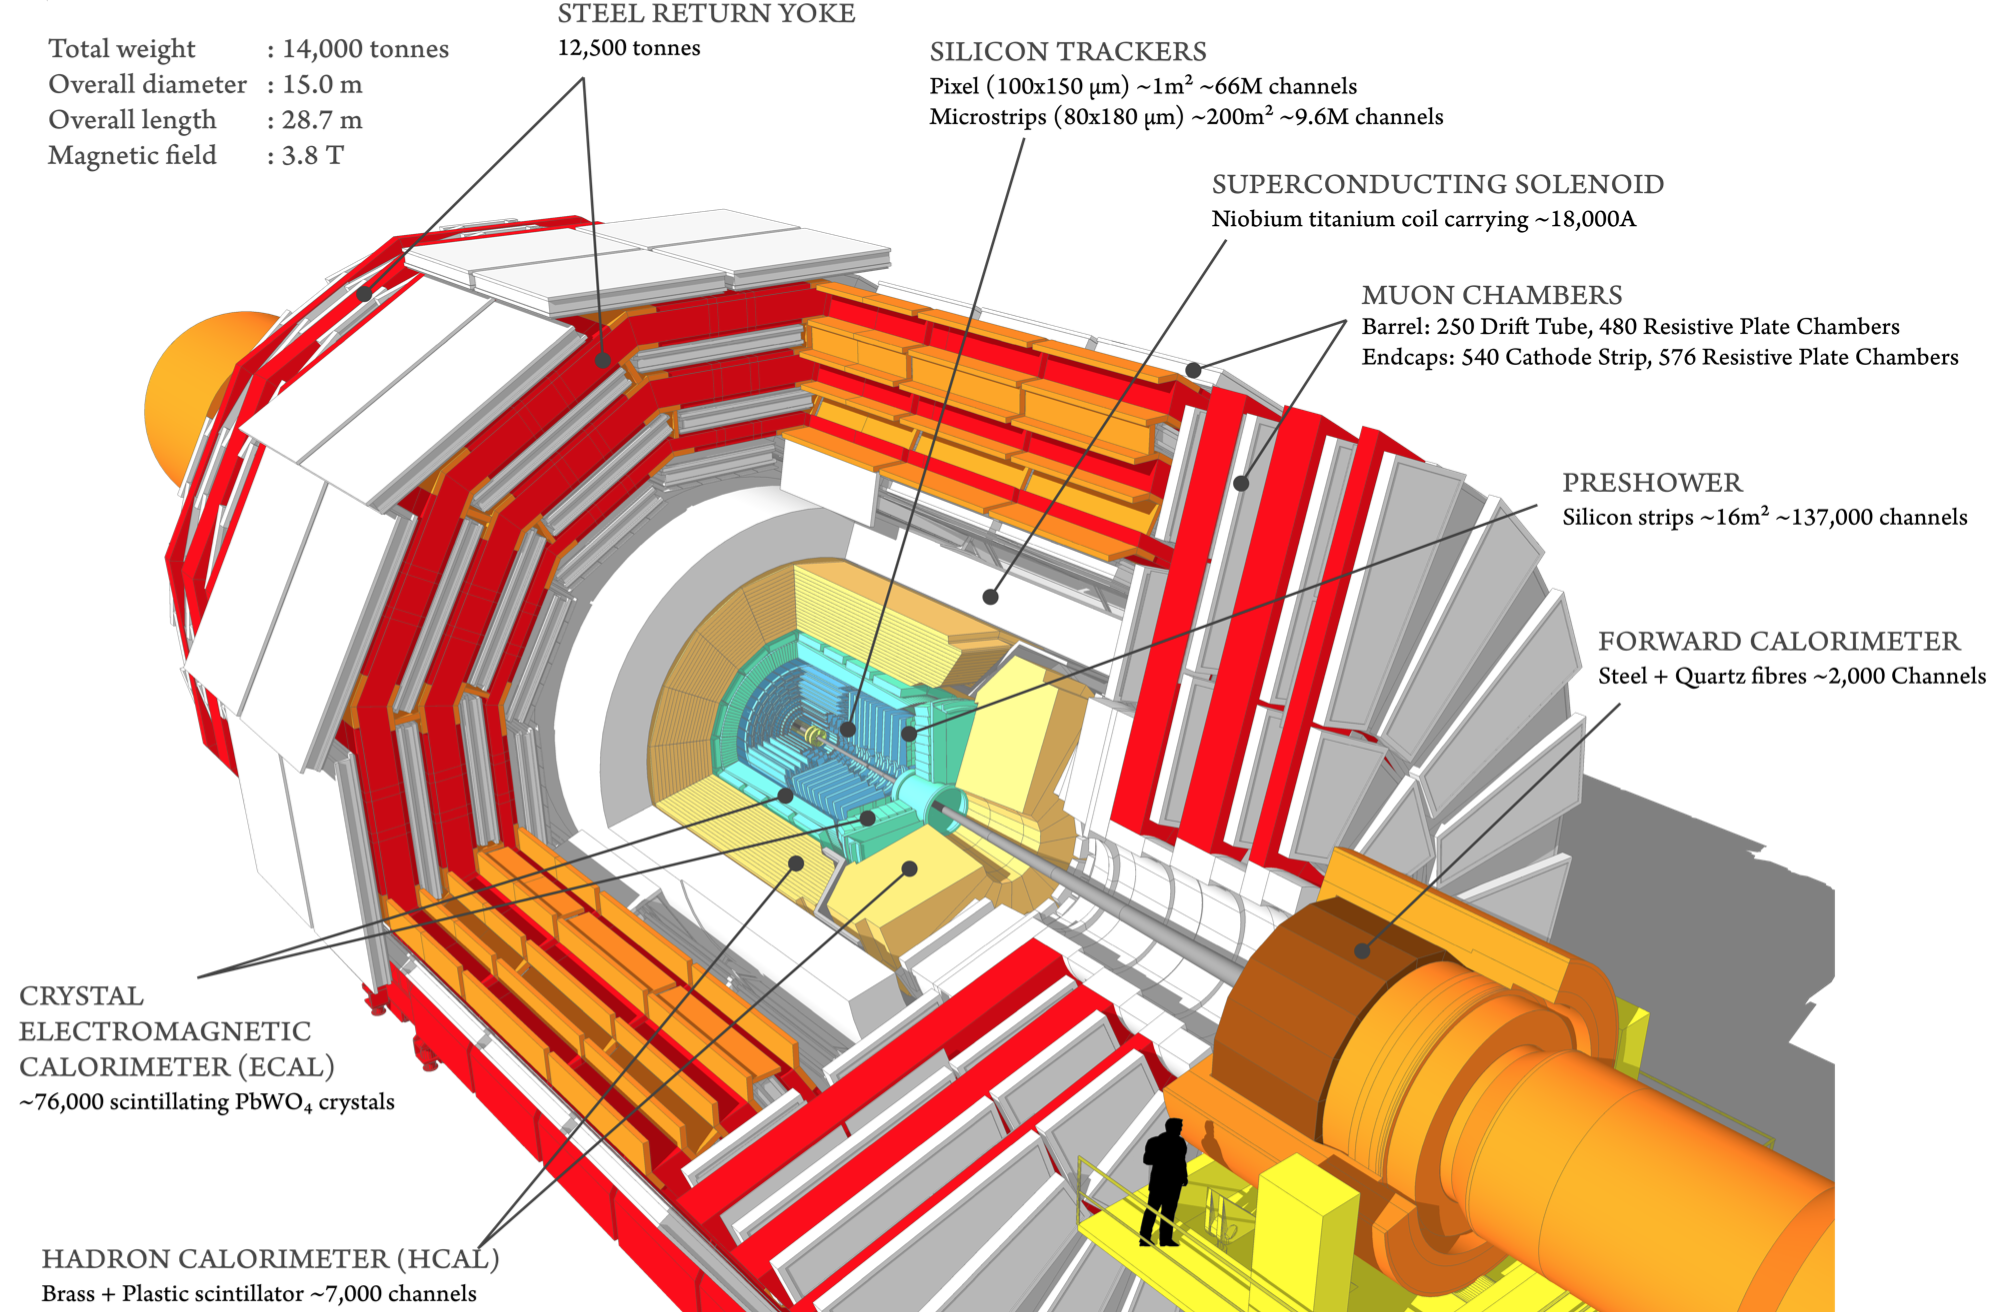
\includegraphics[width=\textwidth]{CMSdetector.png}
	\vspace{2mm}
	\caption[Three dimensional view of the CMS detector showing each component. A human shape is positioned on lower right to compare its size. It is sometimes called as the cylindrical onion due to its shape and concentric layers of components.]
	{Three dimensional view of the CMS detector showing each component. A human shape is positioned on lower right to compare its size. It is sometimes called as the cylindrical onion due to its shape and concentric layers of components \cite{CMSdetector}.}
	\label{CMSdetector}
\end{figure}

\subsection{Structure and the CMS coordinate system}

The CMS detector has a cylindrical shape with a diameter of 15 m and a length of 21.5 m. It contains many detector components in that size that they weigh about 12 500 tonnes and that is another reason for calling it compact. The central region is called \textbf{\emph{barrel}} and each of the forward regions are called \textbf{\emph{endcaps}}. It consists of many concentric layers of sub-detectors for many different purposes, shown in \autoref{CMSdetector}. These layers include, from the innermost part towards outside; a silicon tracker, the electromagnetic calorimeter (ECAL), the hadron calorimeter (HCAL), the superconducting solenoid and the muon chambers. Each component is explained in the following sections. 

The coordinate system of the CMS experiment is a right-handed cartesian system. It accepts the collision point as the centre with the x-axis pointing radially inward to the centre of the LHC's circle, y axis is perpendicular to x-axis and to the direction of the beams which is the z-axis, shown in \autoref{cmscoordinates}. The z-axis points in the anticlockwise direction when looked from above the underground. 

\begin{figure}[ht]
	\centering
	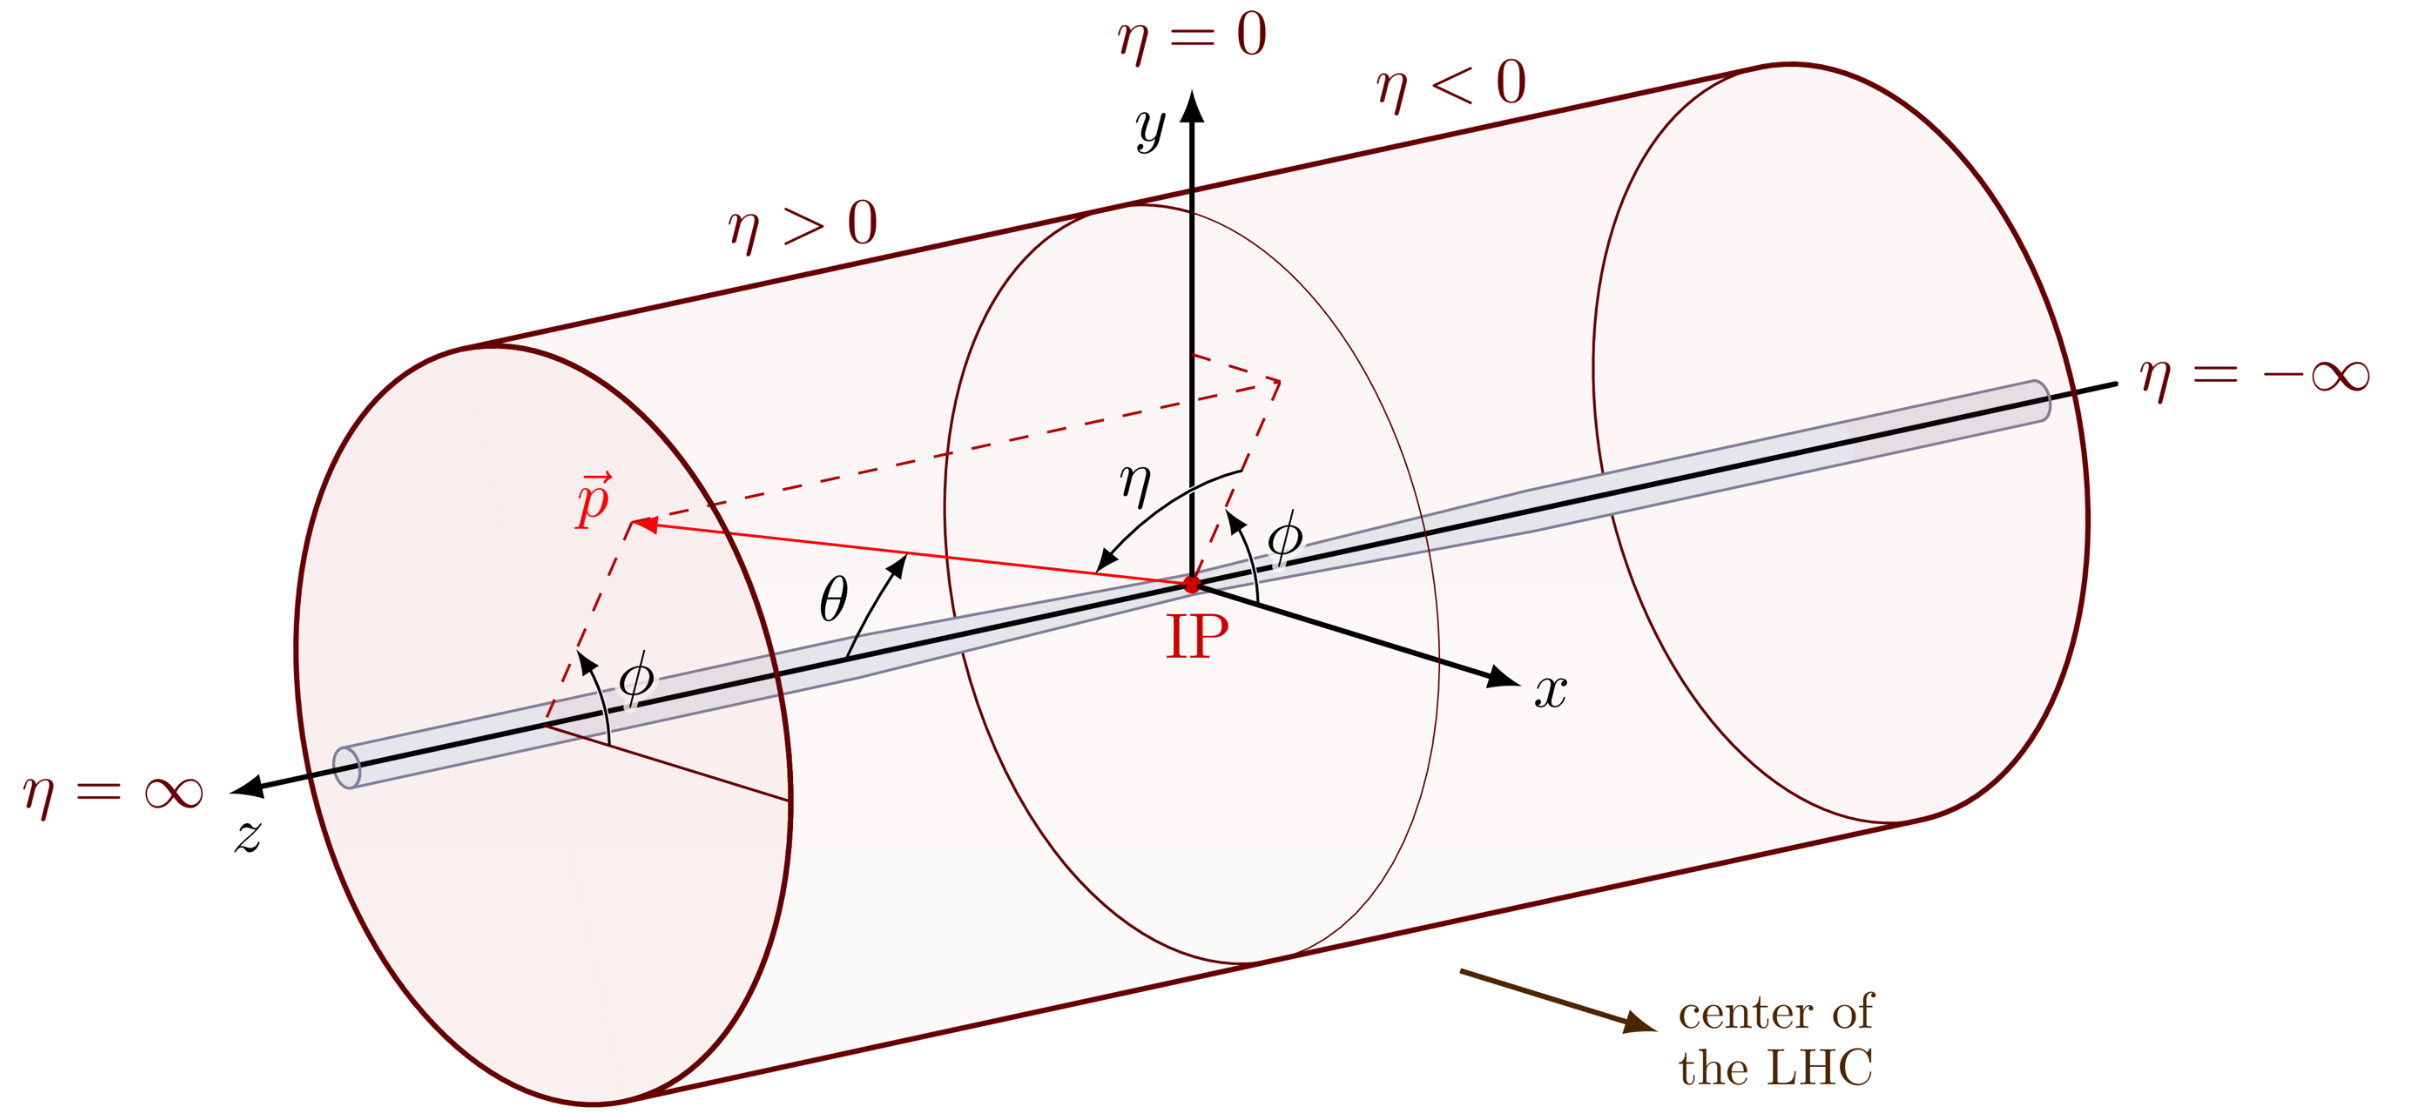
\includegraphics[width=\textwidth]{cmscoordinates.png}
	\vspace{2mm}
	\caption[The coordinate system of the CMS detector. IP denotes the interaction point and the momentum of a particle is shown by $\vec{p}$ in red arrow. Pseudo-rapidity values are shown by $\eta$.]{The coordinate system of the CMS detector. IP denotes the interaction point and the momentum of a particle is shown by $\vec{p}$ in red arrow. Pseudo-rapidity values are shown by $\eta$ \cite{cmscoordinates}.}
	\label{cmscoordinates}
\end{figure}

The cylindrical coordinates is often used for the CMS experiment because of the shape of the detector; an azimuth angle $\phi$ between x and y-axes in $\left[-\pi,+\pi\right]$, and a polar angle $\theta$ between z and y-axes in $\left[0,+\pi\right]$, respectively. Another kinematic quantity, the \textbf{\emph{pseudo-rapidity}} which is a relativistic reference-frame-independent kinetic observable is widely used at the collider physics and defined as $\eta = -ln\left(tan\left(\theta/2\right)\right)$. The barrel region in this reference frame is simply in $|\eta|<1.2$ and two endcaps are in $1.2<|\eta|<3$.

Another kinematic variable, the \textbf{\emph{angular separation}} or angular distance is defined as $\Delta R = \sqrt{\left(\Delta\eta\right)^2 + \left(\Delta\phi\right)^2}$ and is used to separate particles using the cones around the direction of particles. It is also a boost invariant variable. The \textbf{\emph{transverse momentum}}, which is an important kinematic variable in the collider physics, is the projection of the particle's momentum and energy onto the transverse plane that is $\eta = 0$.

\subsection{Solenoid magnet}

The core feature of the CMS detector is the large niobium-titanium superconducting solenoid with 5.9 m inner diameter and 12.5 of length. It creates 3.8 T uniform magnetic field along the beam line axis while operating at 4.5 K with 18 kA of electric current. The magnetic field bends the trajectories of emerging charged particles from the collisions in the transverse plane, see \autoref{cmsdetector2}. It is also useful for measuring the transverse momentum of particles up to TeV/c via the curvatures in their tracks.

\begin{figure}[ht]
	\centering
	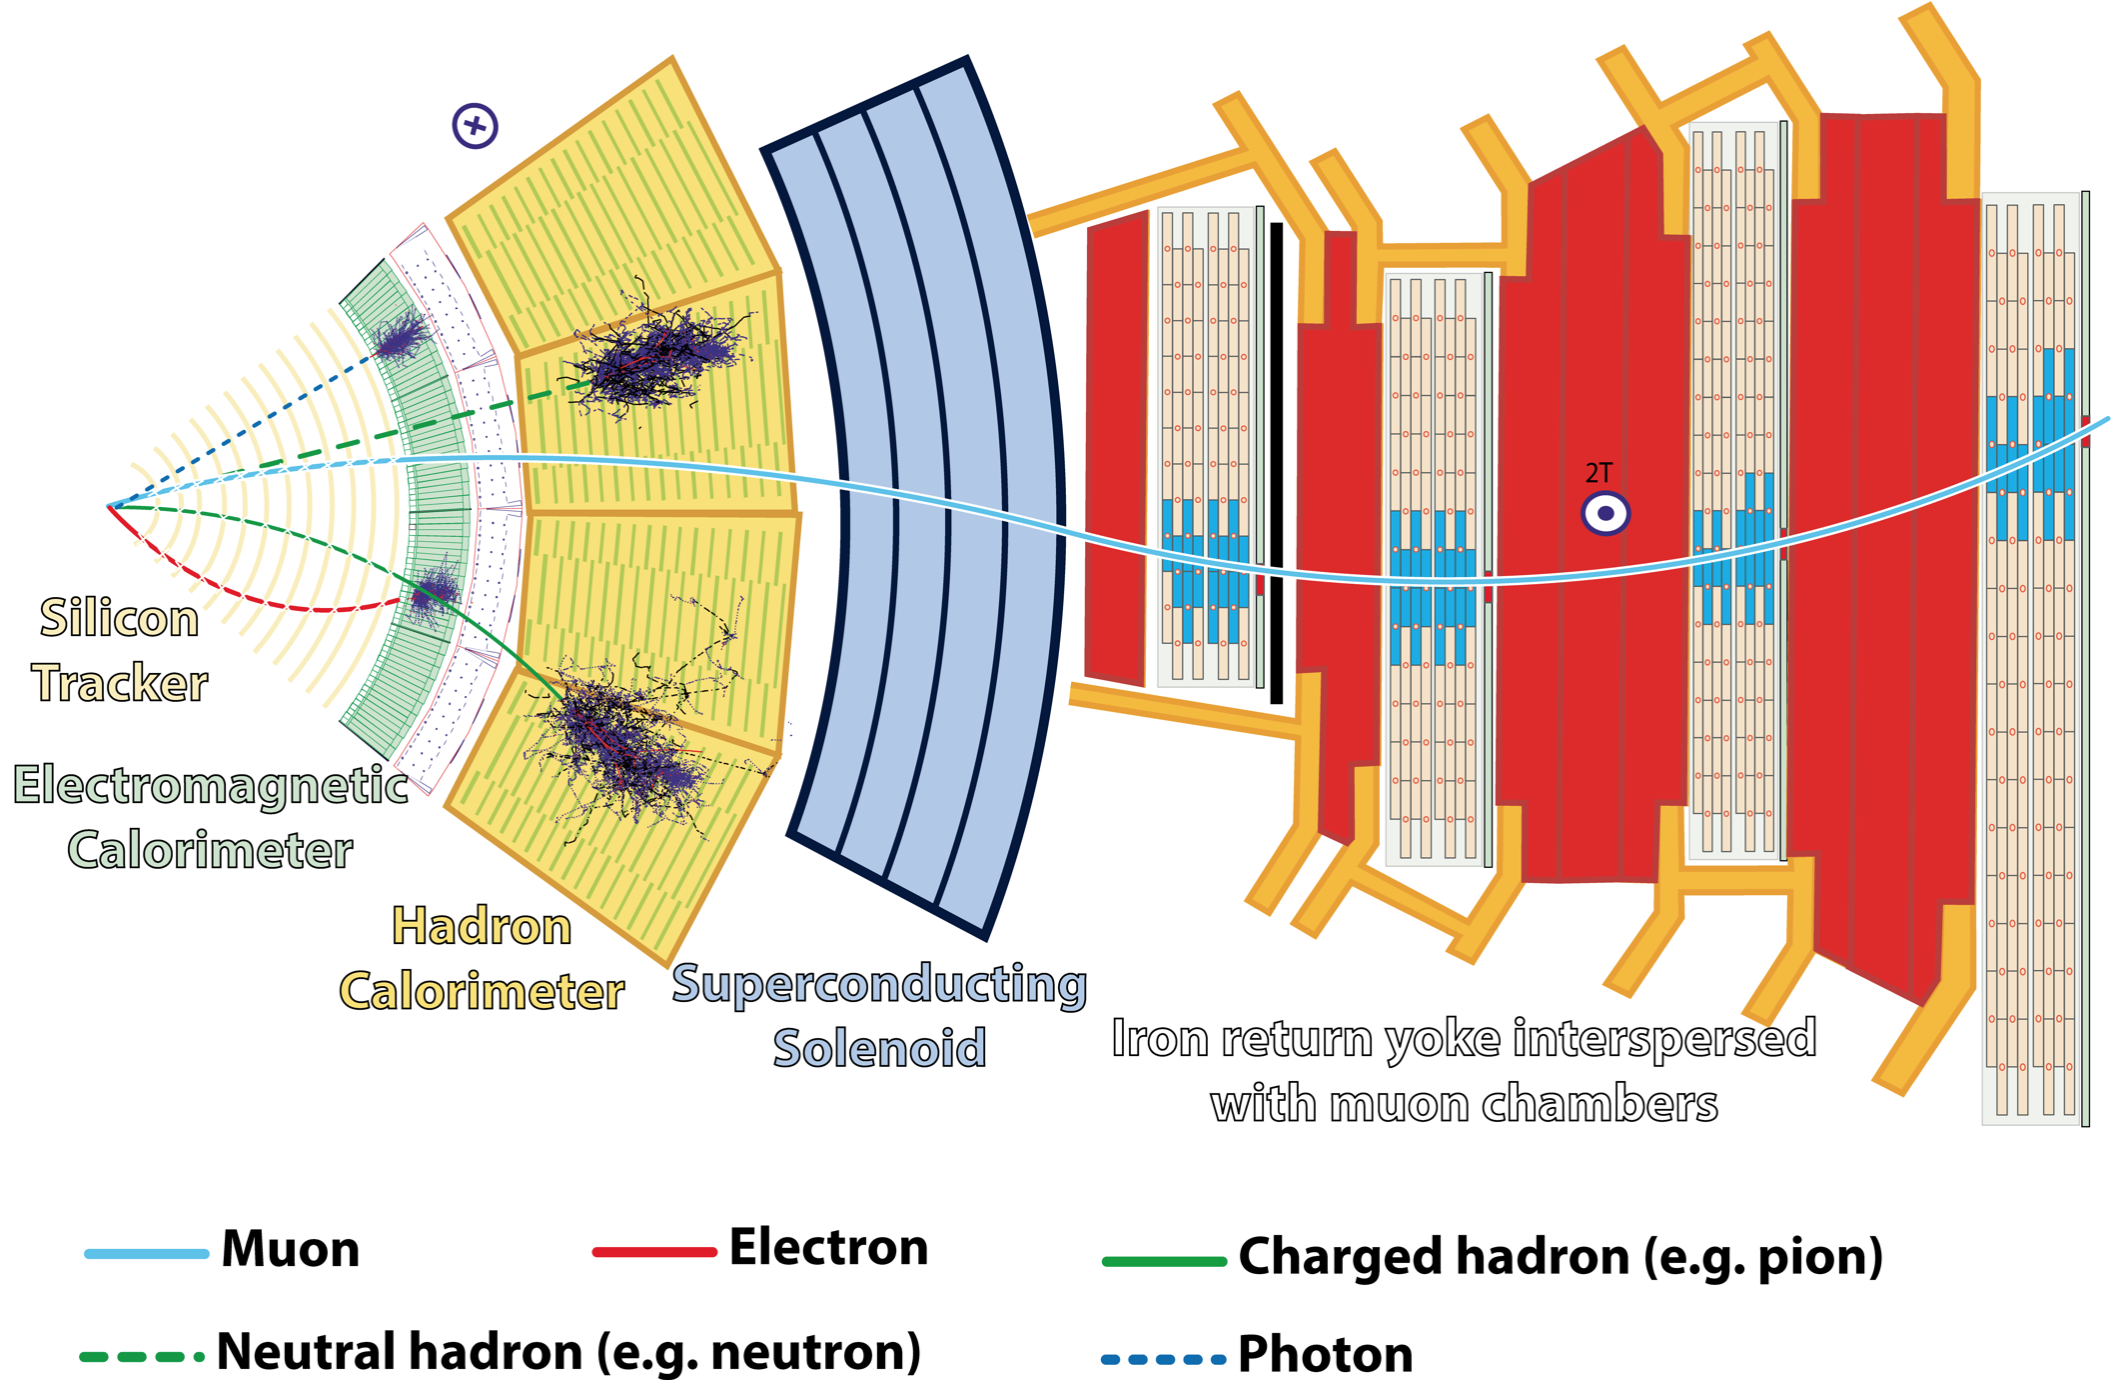
\includegraphics[width=\textwidth]{cmsdetector2.png}
	\vspace{2mm}
	\caption[Schematic view of a transverse slice of the barrel region of the CMS detector. Particles are shown in their trajectories and signatures in the sub-detectors. Photons and electrons create showers in the ECAL but photons don't leave traces in the tracking system which allows to distinguish these two types. The same recognition can be made between neutral and charged hadrons.]{Schematic view of a transverse slice of the barrel region of the CMS detector. Particles are shown in their trajectories and signatures in the sub-detectors. Photons and electrons create showers in the ECAL but photons don't leave traces in the tracking system which allows to distinguish these two types. The same recognition can be made between neutral and charged hadrons \cite{Barney:2120661}.}
	\label{cmsdetector2}
\end{figure}

The solenoid hosts the tracker and calorimeter systems inside it and this requires these sub-detectors to be very compact. The returning magnetic field of the magnet is used to measure the transverse momentum using the muon chambers positioned inside the iron structure surrounding the solenoid and has 2 T of magnetic field. Hence the muons are bent in opposite directions depending on being inside and outside of the solenoid.

\subsection{Inner tracking system}

The first sub-detector system that the emerging particles encounter, is the inner tracking system in $\eta < 2.5$ region. The hitting points in the tracker system of outgoing particles from the interaction point are combined to create a high resolution charge and momentum information. The resolution of these measurements decreases with the increasing transverse momentum since the curvature becomes more straight. The measurements in the inner tracking system also helps to determine the interaction point of hard scatterings, usually known as the \textbf{\emph{primary vertex}}, and its separation from pileup in the event. The reconstruction of additional decays are also performed using the inner tracker, such a B meson decay from the secondary vertex.

In order to provide a radiation durability, the material inside the inner tracking system is kept minimum since the system is the first encounter of the propagating particles from the interaction point; and to limit the energy loss of those particles via coulomb scattering, bremsstrahlung or nuclear interactions before they reach the aimed sub-detector. These requirements are achieved by fast readout on-board electronics for the whole sub-detector consisting two different silicon sensors sensitive to the charged particles shown in \autoref{innertracker}.

\begin{figure}[ht]
	\centering
	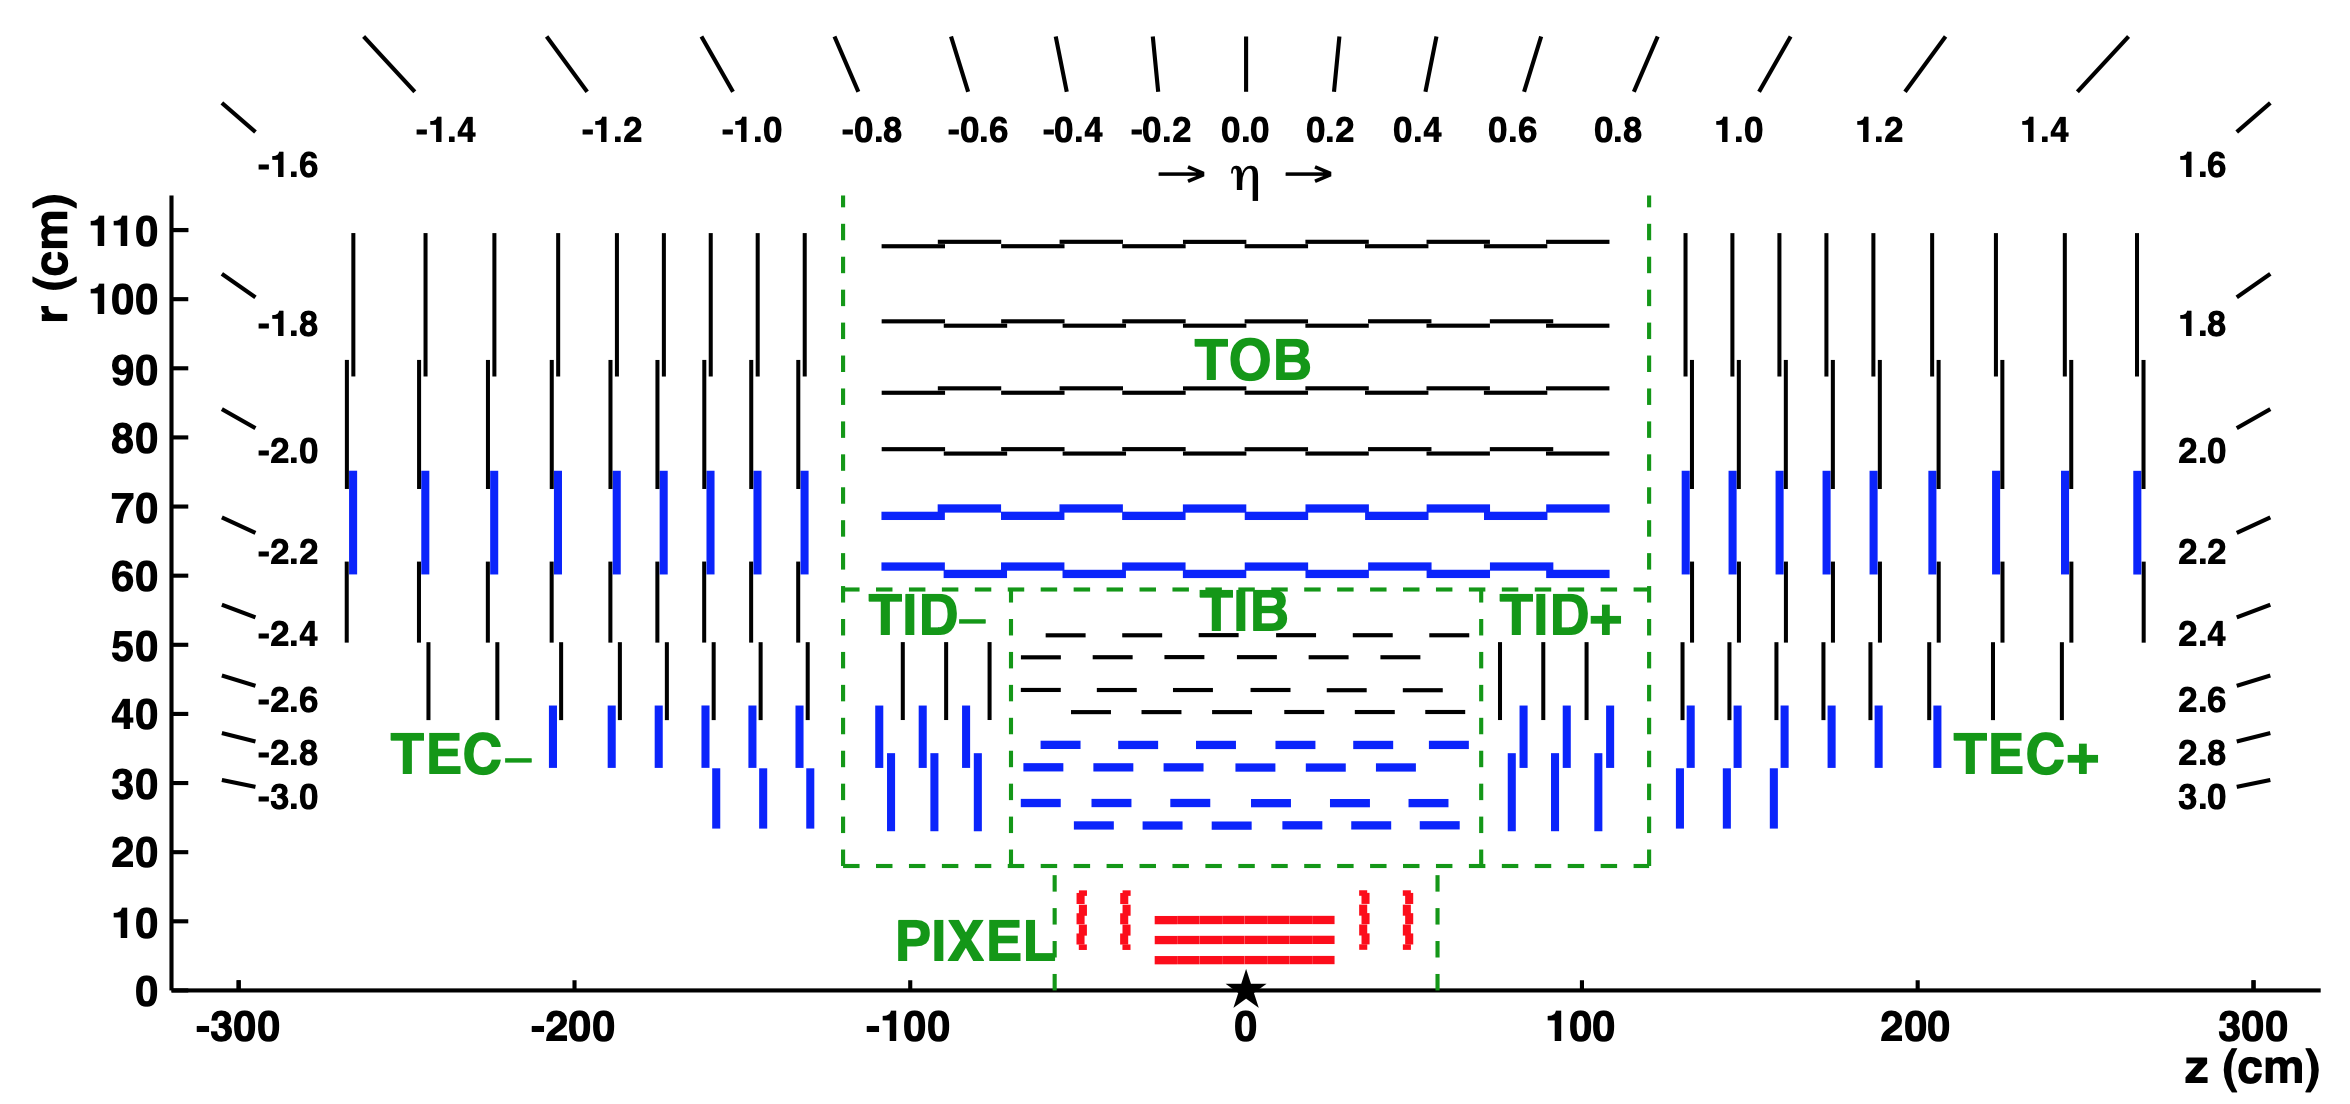
\includegraphics[width=\textwidth]{innertracker.png}
	\vspace{2mm}
	\caption[Schematic cross section of the tracker in the r-z plane with one half shown since the tracker is symmetric about the r = 0. The star indicates the centre of the tracker and the expected collision point. The detector modules are kept in green dashed lines, namely; Tracker inner barrel (TIB) and Tracker inner disks (TID) surrounded by the Tracker outer barrel (TOB) and tracker endcaps (TEC) on the sides. Thin black lines show the strip tracker modules that create 2-D hits, while thick blue lines show the one allowing providing 3-D hit positions which is actually two back-to-back strip modules. The pixel modules provide 3-D hits and they are shown in red curly lines. Each module in a given layer is shifted slightly cover all the gaps providing best acceptance.]{Schematic cross section of the tracker in the r-z plane with one half shown since the tracker is symmetric about the r = 0. The star indicates the centre of the tracker and the expected collision point. The detector modules are kept in green dashed lines, namely; Tracker inner barrel (TIB) and Tracker inner disks (TID) surrounded by the Tracker outer barrel (TOB) and tracker endcaps (TEC) on the sides. Thin black lines show the strip tracker modules that create 2-D hits, while thick blue lines show the one allowing providing 3-D hit positions which is actually two back-to-back strip modules. The pixel modules provide 3-D hits and they are shown in red curly lines. Each module in a given layer is shifted slightly to cover all the gaps providing best acceptance.\cite{innertracker}.}
	\label{innertracker}
\end{figure}

The inner tracker includes a \textbf{\emph{silicon pixel sub-detector}} consisting of four barrel and three endcap pixel detectors. The endcap pixel detectors are in disk shapes and have pixel cells of 100 $\mu m$ x 150 $\mu m$ size providing a resolution of 10 $\mu m$ in the transverse plane, 20 $\mu m$ along the beam axis with the third coordinate being the position of each sensors. A total of 66 million pixels \cite{innertracker} allow highly precise measurements and a high resolution of the impact parameter, the closest distance from the primary vertex to a given track, essential for second vertex reconstruction \cite{innertracker2}. The silicons in these pixels are stimulated when a charged particle passes in them. The pixel detectors and the strip tracker operates at -15\textdegree C and -20\textdegree C, respectively, which reduces the radiation damage and dissipates the heat generated by the on-board electronics. An upgrade of the pixel detector has been performed during the technical stop in 2016 in order to retain its performance which reduced due to radiation damage \cite{tracker3}.

The outermost part of the tracker consists of silicon micro-strips and is called the \textbf{\emph{silicon strip sub-detector}}. It contains about 9.3 million strips covering a $198\;m^2$ area in the $\eta < 2.5$ region. It has 10 cylindrical layers in the barrel region close to the pixel detector; four layers of TIB and six layers of TOB, shown in \autoref{innertracker}. Additionally, 24 disks of endcap modules are installed each containing concentric disks of silicon strip modules; three TIDs on the sides of TIBs, and nine TEC disks covering $124<|z|<282\;cm$. \autoref{Mbudget} shows the tracking system's materials budget, which is basically the detector thickness in units of radiation length (the amount of material traversed by particles in the detector).

\begin{figure}[ht]
	\centering
	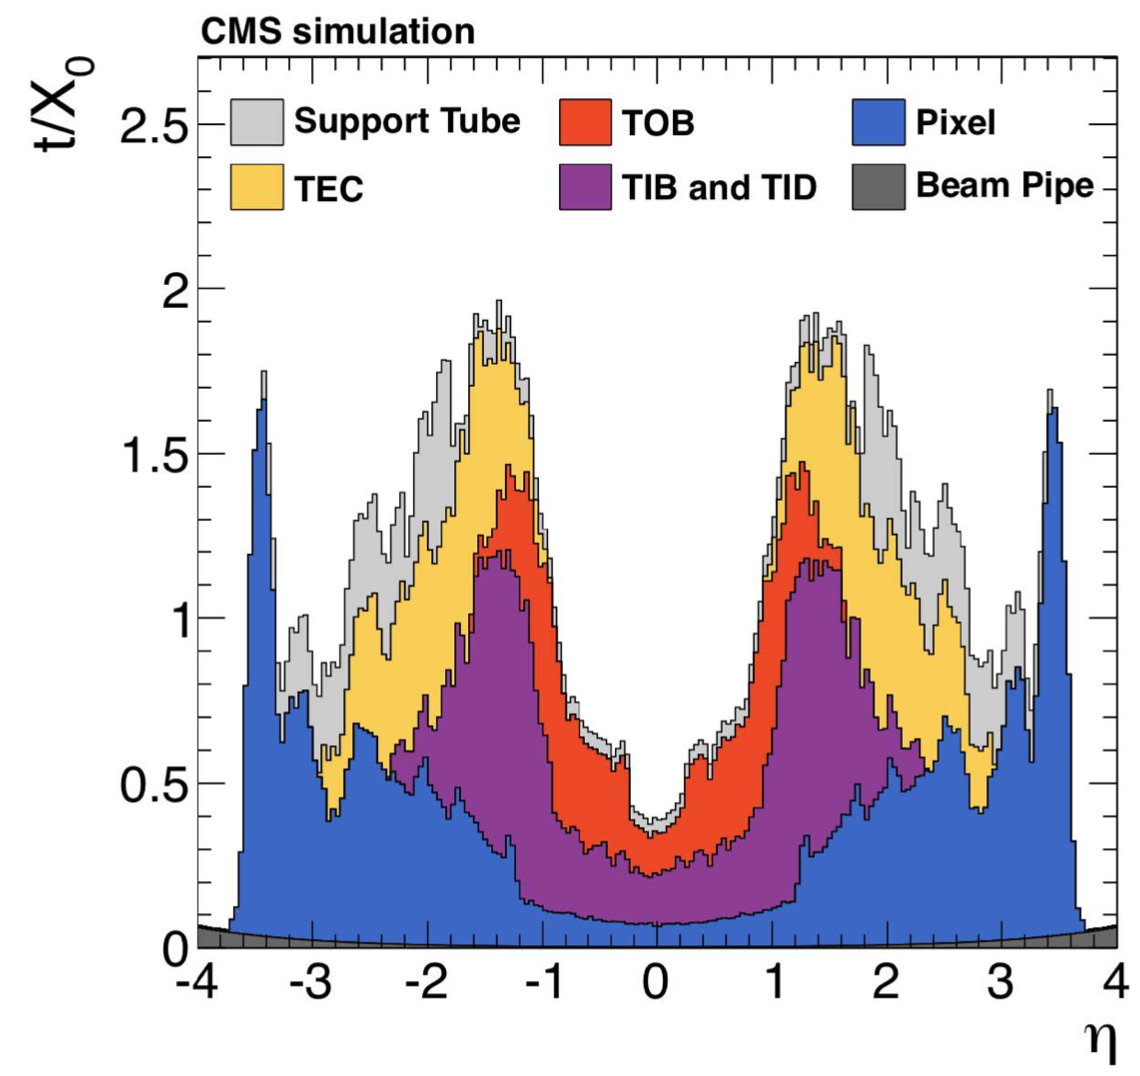
\includegraphics[scale=0.6]{Mbudget.png}
	\vspace{2mm}
	\caption[The material budget contribution from sub-systems as a function of $\eta$, showin the tracker sub-detectors, beam pipe and the supper tube that surrounds the tracker.]{The material budget contribution from sub-systems as a function of $\eta$, showin the tracker sub-detectors, beam pipe and the supper tube that surrounds the tracker \cite{Mbudget}.}
	\label{Mbudget}
\end{figure}

\subsection{Electromagnetic calorimeter}\label{ecalsubsection}

The calorimeters are designed to measure the energy of both charged and neutral particles by their interaction with the detector material. The ECAL \cite{CERN-LHCC-97-033} performs the energy measurements of electrons and photons. It is placed between the tracker and the HCAL, and is highly granular made up of lead tungstate inorganic crystals ($PbWO_4$). The energy measurement is made by a photosensitive device in the ECAL, that is excited by the scintillation light coming from the interaction of the crystal material with an electromagnetic shower originating from an incident electron or muon.

The ($PbWO_4$) is a good material choice here because of its short Moli\`ere radius, that is the radius approximately of a cylinder coaxial with the shower axis which contains 90\% of the energy of the shower. It means that the crystal material can contain the EM shower. Besides, ($PbWO_4$) is good scintillating medium with a small radiation length which is useful for determining the amount of depth of material traversed by particles. Additionally, lead tungstate is a radiation hard material; almost 80\% of the scintillation happens within 25 ns. The very short scintillation time is also an essential feature given the high luminosity of the LHC and bunch spacing. A drawback of this material is its low light yield, which requires using extra amplification.

The barrel of the ECAL (EB) contains 61 200 crystals in $|\eta|<1.479$ region and two endcaps (EE) are made up of about 7300 crystals covering $|\eta|<3.0$ shown in \autoref{cal}. The crystals in both EB and EE are aligned such that their axes confronts the nominal interaction point ensuring the escape of particles to a minimum. The scintillation light coming from the interaction of the particles with the crystals is read-out by avalanche photo-diodes in EB and by vacuum photo-triods in two EEs, and the ECAL as a whole operates at 18 \textdegree C.

\begin{figure}[ht]
	\centering
	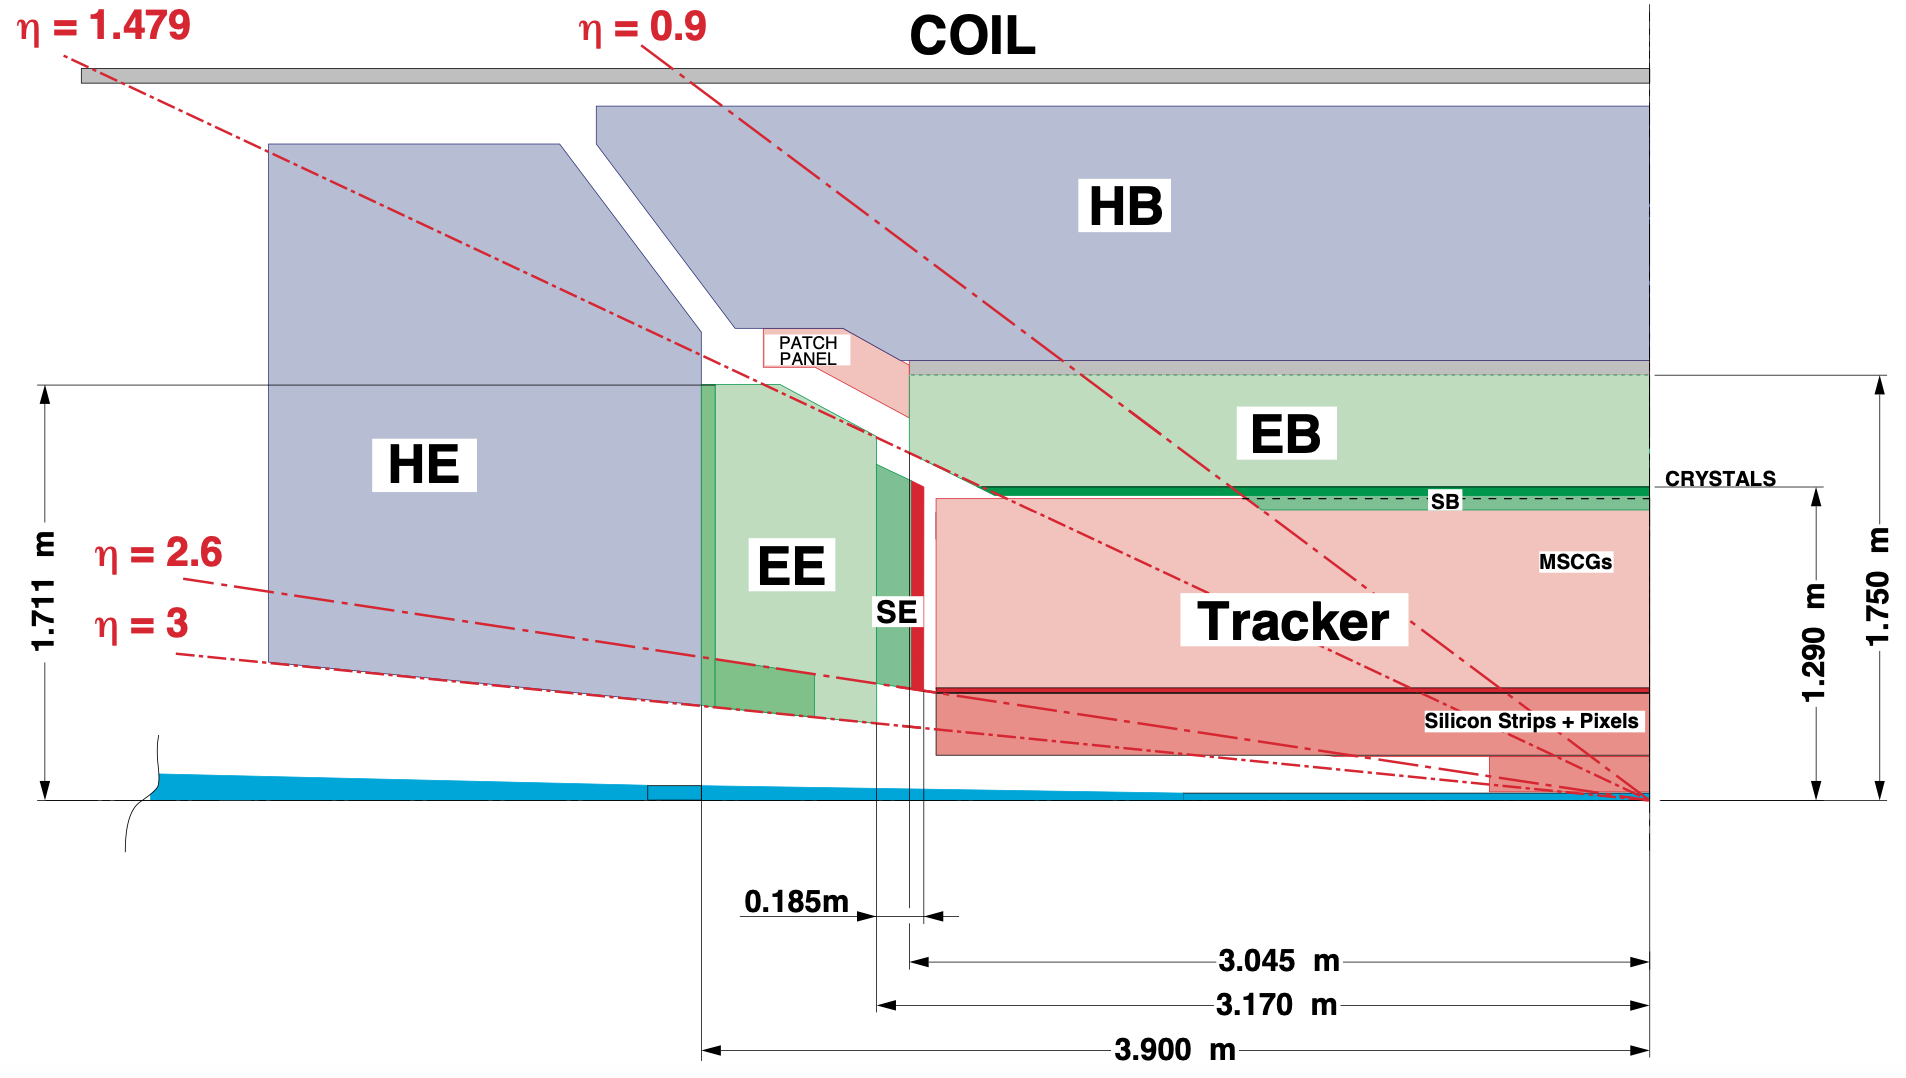
\includegraphics[width=\textwidth]{cal.png}
	\vspace{2mm}
	\caption[Schematic view showing one quadrant of the calorimetry and tracking system.]{Schematic view of one quadrant of the calorimetry and tracking system \cite{CERN-LHCC-97-033}.}
	\label{cal}
\end{figure}

Two EM pre-shower (ES) sampling sub-detectors are installed in the front sides of the EEs, each containing a sampling calorimeter consisting two lead layers to initiate EM showers. These lead layers are followed by 2-mm silicon strip detectors to measure the transverse profile of the showers. They provide 2-D profiling of the showers thanks to their orthogonal placement.

The energy resolution of the ECAL barrel was measured in 7 TeV data using electron from $Z \rightarrow e^+e^-$ decays, resulting an energy resolution better than 2\% in $|\eta|<0.8$ and ranging from 2 to 5\% in other regions \cite{ecalm}. Energy resolution formula for the ECAL reads;
\be
\left(\frac{\sigma}{E} \right)^2 = \left(\frac{S\left(\eta\right)}{\sqrt{E}} \right)^2 + \left(\frac{N\left(\eta\right)}{E} \right)^2 + C\left(\eta\right)^2 \; .
\label{res_eq_ecal}
\ee

The energy resolution of a calorimeter increases with the particle energy because of the reduction in the first and the second terms in the equation. The first term is called \emph{\bf{stochastic term}} and is proportional to the number of photons caused by the scintillation in the interactions. The second term is the \emph{\bf{noise term}} and signifies the noise originating from the electronic readout systems. Finally, the third term, being a constant, depends on the detector inhomogenities, calibration uncertainties and some instrumental effects. The values for ECAL are measured for ECAL barrel during a test beam with incident electrons as $2.8\%$, $41.5 \; MeV$ and $0.3\%$, respectively \cite{Ingram2007}.

\subsection{Hadron calorimeter}

The HCAL\cite{CMS:1997xji} is designed to absorb hadrons coming from the collisions which usually pass the ECAL without being stopped. The energy of the hadrons are measured from their showers in the HCAL, which is a more difficult task than the one made in ECAL about the electrons and photons because of rare effects in the shower generation where many undetectable particles may be produced from nuclear and hadronic interactions. These effects reduces the energy resolution of the hadrons detected in the HCAL, on the other hand the particle flow reconstruction techniques can improve the resolution offline, explained in \autoref{ch3}.

The HCAL is at the heart of the reconstruction of jets produced in the final states. It is made up of two main sections; a barrel (HB) and two endcaps (HE) \autoref{cal} covering $|\eta|<1.3$ and $|\eta|<3.0$, respectively. These two sub-detectors are sampling calorimeters each containing a brass absorber made up of 70\% copper and 30\% Zinc and active plastic scintillating tiles between the absorbers. The choice of the brass was due to its paramagnetic character along with other aspects. The light coming from the scintillation is gathered in wavelength shifting fibres (WLFs) which are embedded in the tiles. The WFLS alter the frequency of the coming light to dispatch the light to hybrid photo-diodes (HPDs). The read-out units are composed of scintillating tiles with dimensions of $0.087x0.088$($\Delta\eta x\Delta\phi$) in the HB and of $0.17x0.17$ in the HE.

An outer layer (HO) is placed on the outer surface of the solenoid using iron as observer which extends the total interaction depth to 11 times of the average interaction depth of hadrons in the HCAL. The interaction depth here indicates the nuclear interaction length meaning the distance travelled by a hadron before being submit to an inelastic nuclear interaction.

Another part of the hadronic calorimetry system is the very forward calorimeter (HF). Two HFs are placed 11.2 m away from the interaction point in each direction along the beam line and cover the pseudorapidity range $3<|\eta|<5$. The HF is very useful in reconstructing the very forward jets and is crucial to measure forward jets produced in VBF Higgs production. Since the radiation level is very high in this region, these sub-detectors are equipped with radiation-hard steel absorbers and quartz fibres. The quartz fibres produce Cherenkov radiation which is measured by photomultiplier tubes (PMTs). Two different lengths of fibres are installed in order to distinguish the EM showers from hadronic showers; an EM shower leaves a large fraction of its energy in the first 22 cm of the calorimeter whereas a hadronic shower leaves equal amount of trace along the HF. A general view of the HCAL can be seen \autoref{hcal}.

\begin{figure}[ht]
	\centering
	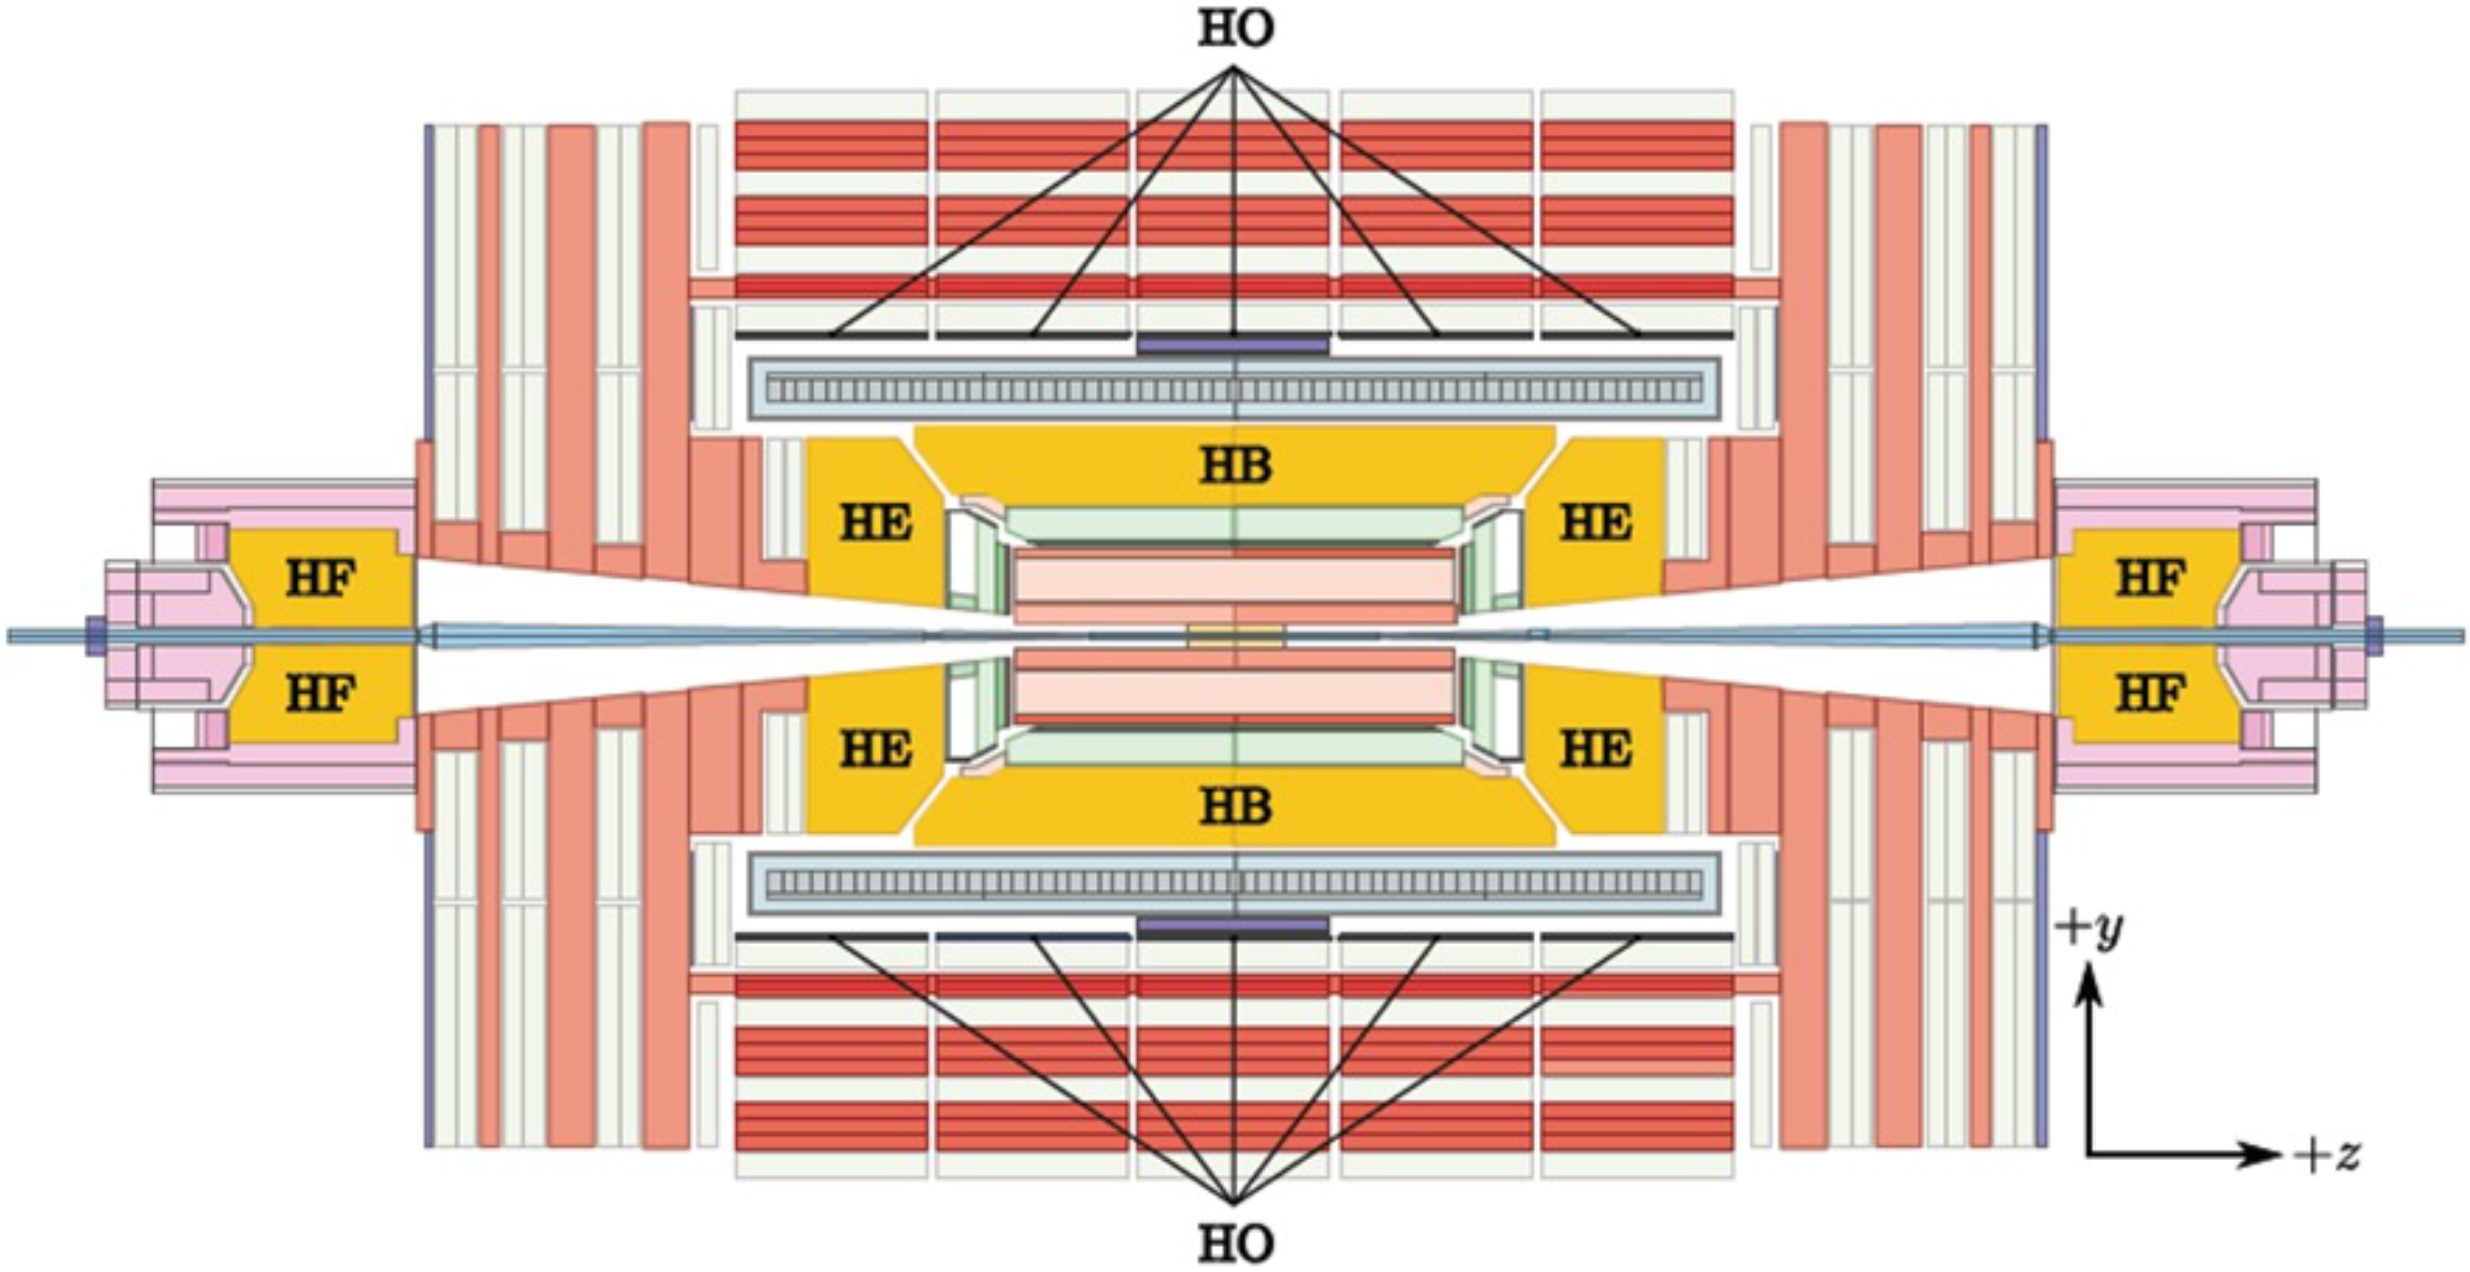
\includegraphics[width=\textwidth]{hcal.png}
	\vspace{2mm}
	\caption[Schematic view of the CMS detector in the y-z plane with the HCAL sub-detectors labelled.]{Schematic view of the CMS detector in the y-z plane with the HCAL sub-detectors labelled \cite{CMS-PHO-GEN-2012-002}.}
	\label{hcal}
\end{figure}

\subsection{Muon system}

The typical energy of muons allow them to pass the ECAL, the HCAL and the solenoid without being stoppped. The muon sub-detectors constitute the outermost part of the CMS detector, and identify the radiating muons and measure their properties such as $p_T$ and charge. It also provides a powerful trigger for events that involve muons and accurate time measurement of the bunch crossing \cite{Layter:343814}.

The muon system is positioned just outside of the solenoid magnet covering the $|\eta| < 2.4$ region, and is interspersed with the iron return yokes in order to bend the trajectory of muons hence to measure their $p_T$, with the 3.8 T magnetic field inside the solenoid and the 1.8 T average return field. Additionally, the muon systems are well protected from the charged particles other than muons due to the presence of a large amount of material including the solenoid.

The  muon system consists of three types of gaseous detectors; Drift Tubes (DTs), Cathode Strip Chambers (CSCs) and Resistive Plate Chambers (RPCs). The DTs are placed within $|\eta| < 1.2$ region in the barrel, the CSCs in $0.9<|eta|<2.4$ in the endcaps and the RPCs in both barrel and endcaps, shown in \autoref{muon1}. Each of these gaseous detectors is placed in a particular region in the detector due to their different rate capabilities which is a parameter related with the time needed for the material to receive the next particle, and due to the ability to work inside a magnetic field.

\begin{figure}[ht]
	\centering
	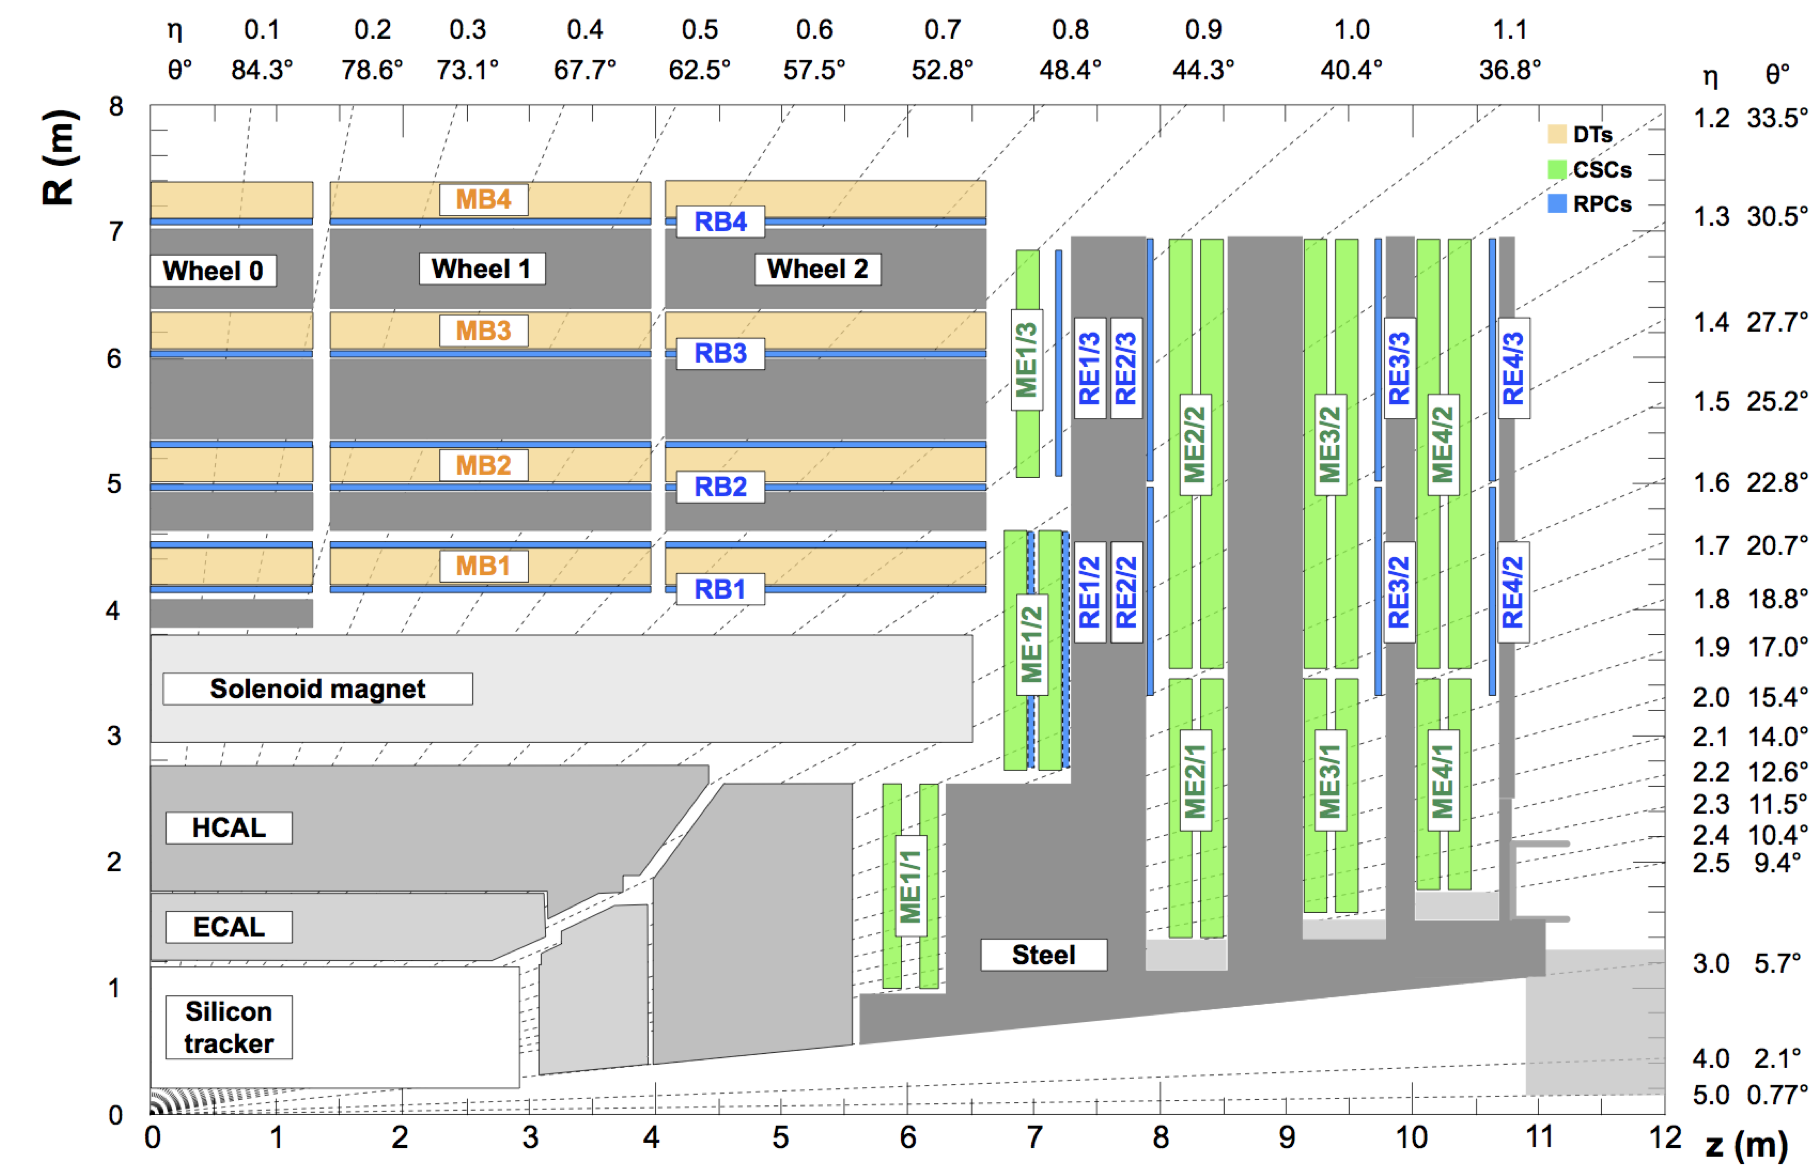
\includegraphics[width=\textwidth]{muon1.png}
	\vspace{2mm}
	\caption[R-z cross section of a quadrant of the CMS detector. The bottom left corner indicates the interaction point. Various muon stations and the steel flux-return disks are shown. The drift tube stations (DTs) are labelled MB (Muon Barrel) and the cathod strip chambers (CSCs) are labelled ME (Muon Endcap). The resistive plate chambers in the barrel and in the endcaps are shown RB and RE, respectively.]{R-z cross section of a quadrant of the CMS detector. The bottom left corner indicates the interaction point. Various muon stations and the steel flux-return disks are shown. The drift tube stations (DTs) are labelled MB (Muon Barrel) and the cathod strip chambers (CSCs) are labelled ME (Muon Endcap). The resistive plate chambers in the barrel and in the endcaps are shown RB and RE, respectively\cite{muon1}.}
	\label{muon1}
\end{figure}

These limitations require the \emph{\textbf{Drift Tubes}}, which do not have a high rate capability, to be placed only in the barrel region. Also the DTs require the trajectory of the particles traversing them modified as small as possible. This makes the barrel is a good choice, where the residual magnetic field is low. Another advantage of placing DTs in the barrel is that the muon and neutron induced background rates are low. The Muon Barrel (MB) detectors consist of four stations in coaxial cylindrical layouts around the beamline interspersed with the iron yoke. These cylindrical stations make up the five wheels of stations aligned in the beamline direction with five wheels of return yokes placed in between. This region consists 250 drift chambers.

The basic constituent of a DT is the drift cell, shown in \autoref{drifttubes}, is a tube of rectangular cross section and filled with $Ar/CO_2 (85/15)$ gas mixture. An anode wire is placed in each of the cells, while the cathode strips are positioned along the small sides. When a charged particle is passed through the cell, the atoms of the contained gas becomes ionised and the resulting electrons of the gas atoms drift towards the anode wire. The geometry of the cell provides a uniform electric field inside which allows the drift velocity to be constant and precise, it is possible to measure the drift time of the electrons therefore the position of the ionising particle \cite{Sirunyan_2018}.

\begin{figure}[ht]
	\centering
	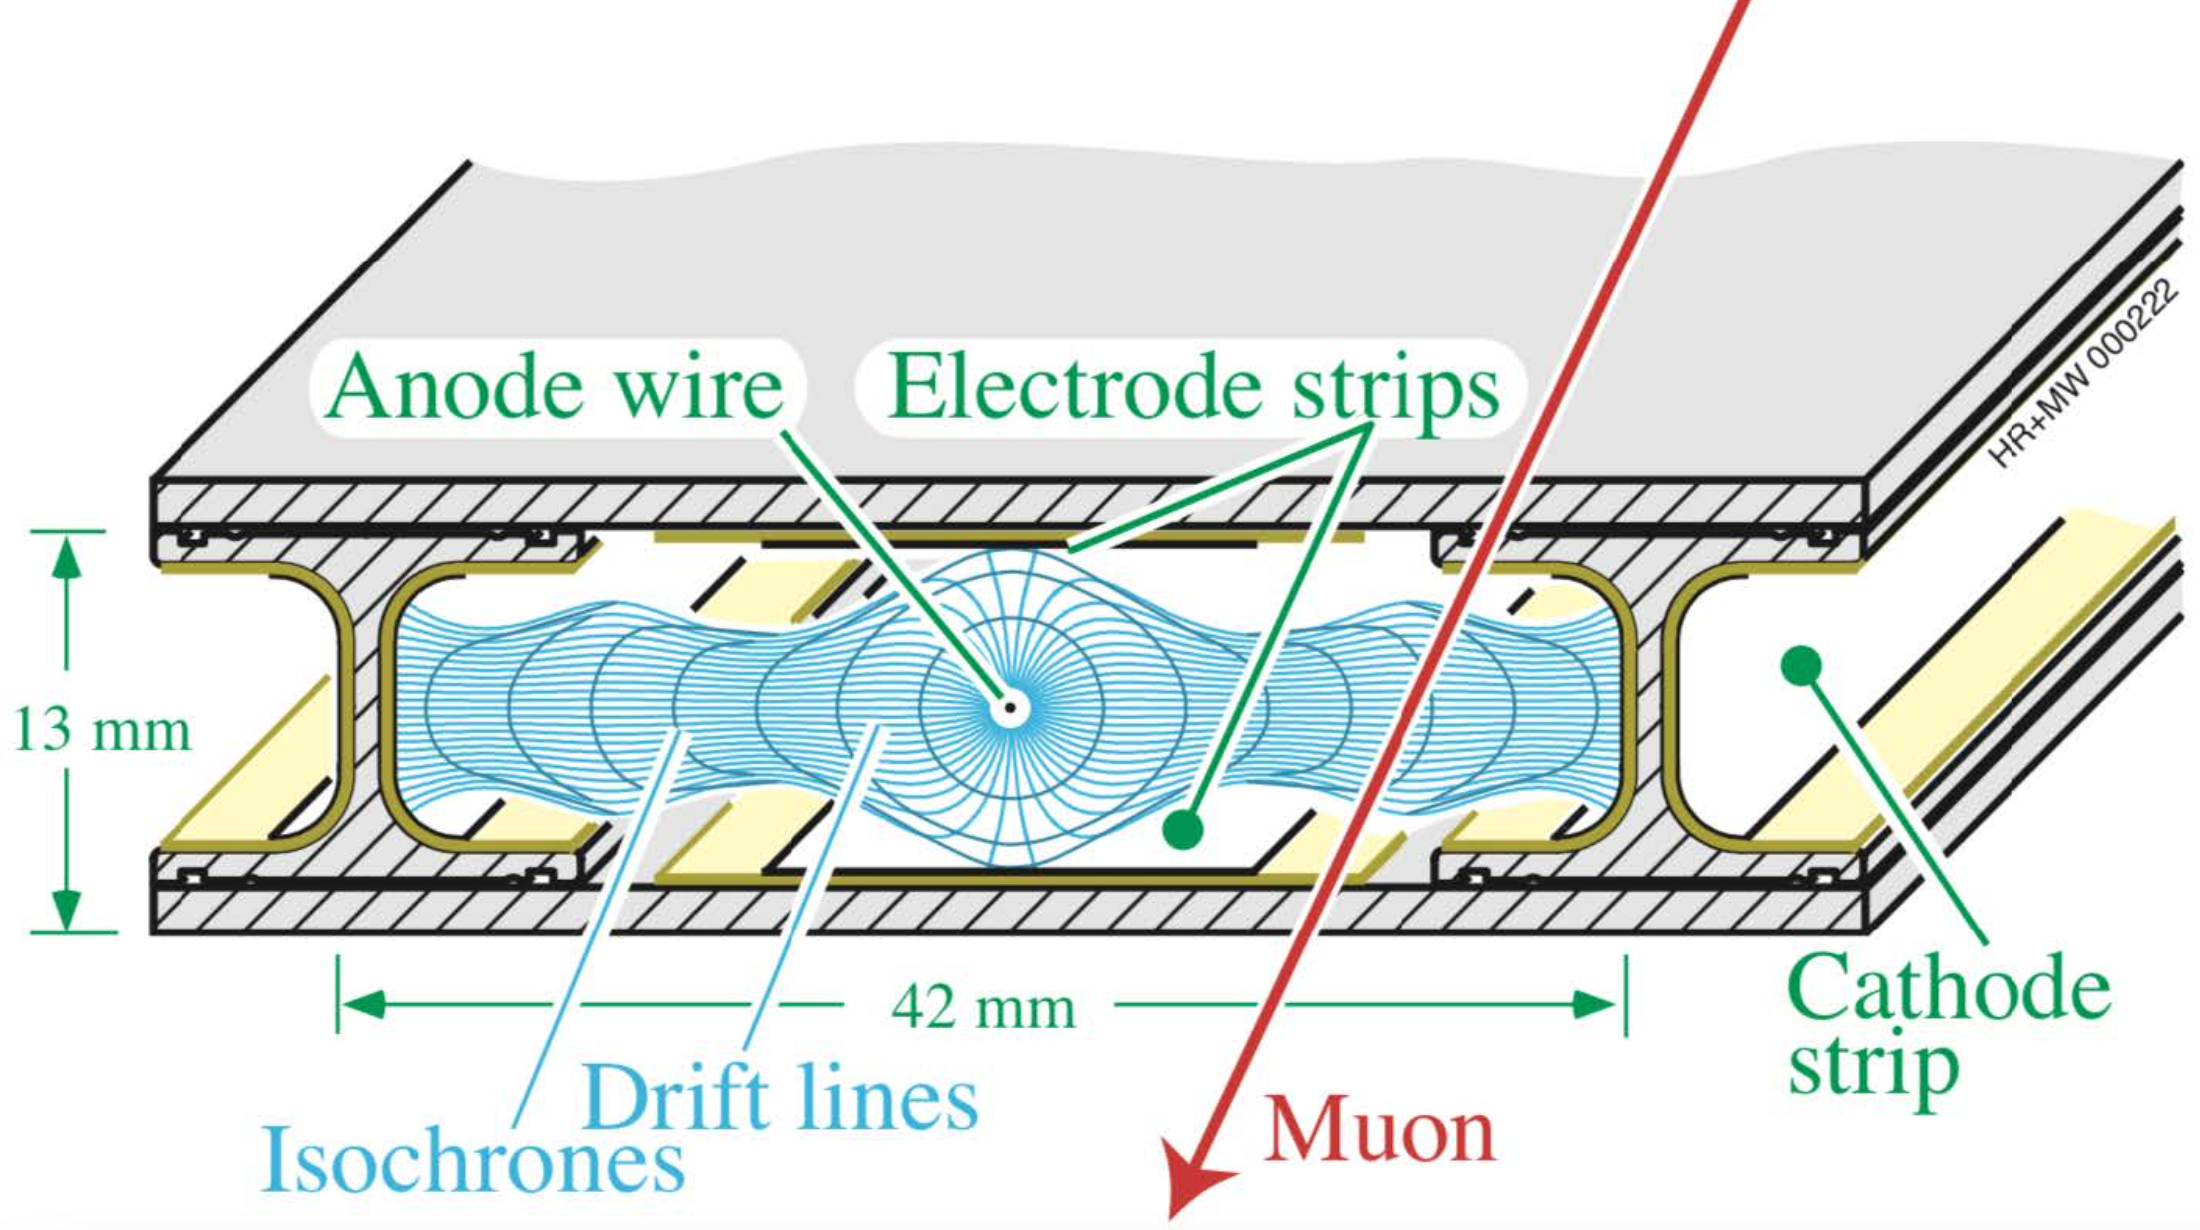
\includegraphics[width=\textwidth]{drifttubes.png}
	\vspace{2mm}
	\caption[Schematic view of a drift cell showing the electric field lines in the gas volume as well as the isochrones (contours of equal drift times) and the drift lines.]{Schematic view of a drift cell showing the electric field lines in the gas volume as well as the isochrones (contours of equal drift times) and the drift lines \cite{Abbiendi:2705998}.}
	\label{drifttubes}
\end{figure}

A single drift cell, with a $42 x 13\; mm^2$ cross section and $2-3$ m of wire length, ensures a drift time of about $400\; ns$ and a resolution of about $200\;\mu m$ resulting in $80-120\;ns$ of resolution for the global chamber measurement. Four stacked layers of drift cell constitute a super-layer, and two or three super-layers make up a drift tube. The orientation of the anode wire differs; in the outer super-layers they are parallel to the beamline, while they are orthogonal for the inner ones. This arrangement allows to provide information regarding different coordinates; a track measurement is performed in the ($r, \phi$) plane in the outer super-layers where the residual magnetic field is low, while the inner part measures the z coordinate.

Contrary to the DTs, the \emph{\textbf{Cathode Strip Chambers}} are placed in the endcaps where a higher residual magnetic field and larger particle rate is present, since they are more robust for the radiative environment and the magnetic field. Both the DTs and the CSCs yield a high spatial resolution for the $p_T$ measurement of the charged particles. The main task of the CSCs is the tracking measurement of the muons, formed as four stations at each endcap. Each CSC is composed of a multi-wire proportional chamber, where the cathode plane is divided into sections of strips that are perpendicular to the wire direction. The chambers are filled with the $Ar/CO_2/CF_4 (40/50/10)$ gas mixture, they have a trapezoidal shape that is made up of seven cathode planes stacked with a 10 mm gas gap between and contain planes of anode wires, shown in \autoref{csc}. When a muon passes through one of the CSCs, it produces an avalanche of electron-ion pairs in the gas and induces signals on the cathode strip wires. The information is then used to acquire the position of the ionising particle, with the radial component being measured with the wires and the z component via the cathode planes \cite{Sirunyan_2018}.

\begin{figure*}[ht]
	\centering
	\begin{subfigure}[b]{0.475\textwidth}
		\centering
		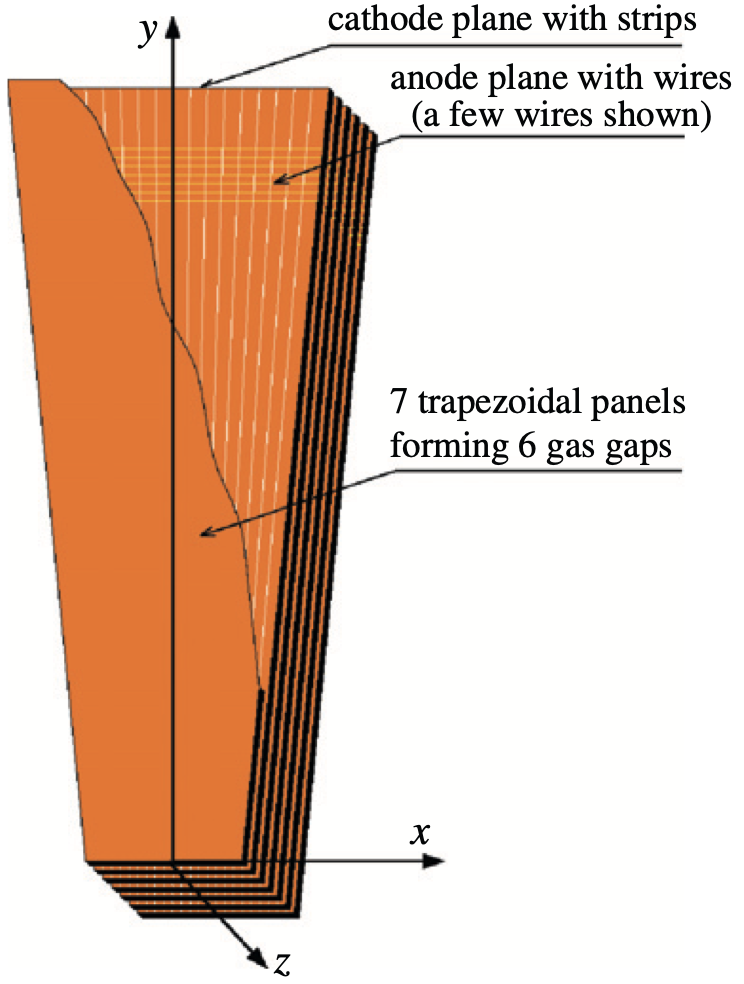
\includegraphics[width=\textwidth]{csc1.png}
		\vspace{-0.75cm}
		\firstsubcaption{CSC}
		\label{csc1}
	\end{subfigure}
	\hspace{0.2cm}
	\begin{subfigure}[b]{0.475\textwidth}  
		\centering 
		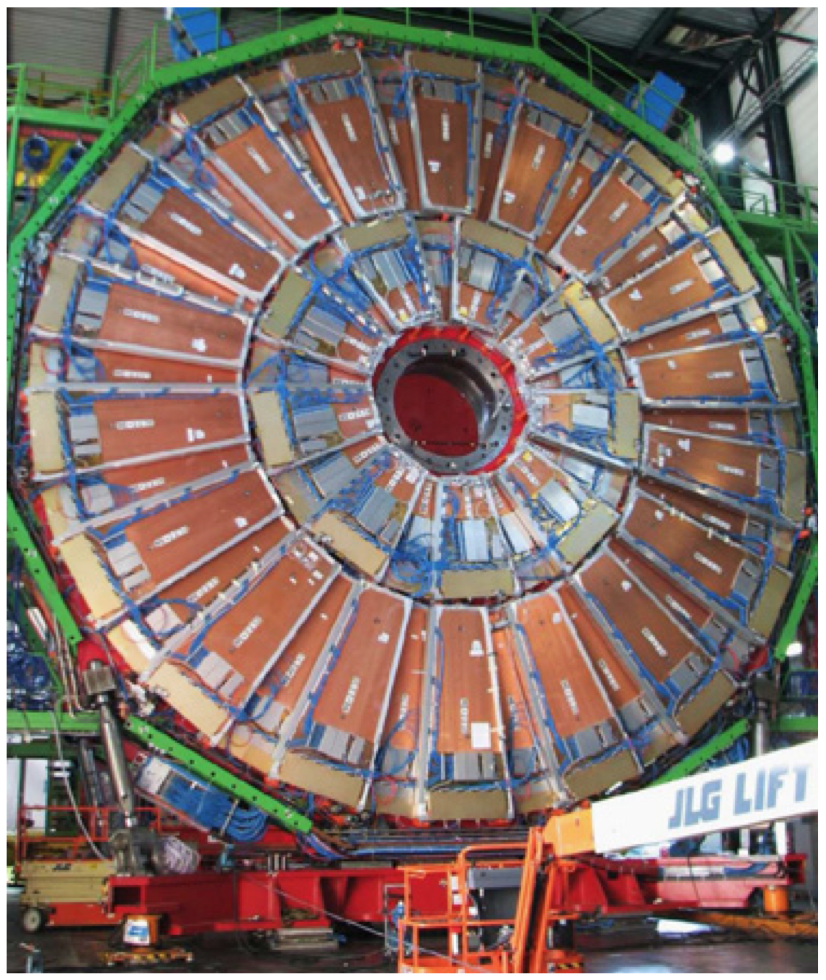
\includegraphics[width=\textwidth]{csc2.png}
		\vspace{-0.75cm}
		\firstsubcaption{CMS Endcap}
		\label{csc2}
	\end{subfigure}
	\caption[Schematic view of a CSC (a) and a photo of the ME+2 disk with its stations of CSCs.]
	{\small (a) Schematic view of a CSC and, (b) a photo of the ME+2 disk with its stations of CSCs\cite{Acosta2008}.}
	\label{csc}
\end{figure*}

Finally, the \emph{\textbf{Resistive Plate Chambers}} are installed in both barrel and endcaps in order to provide a redundancy in the muon chambers with their fast trigger signal. The RPCs constitute 1056 parallel-plate gas detectors with a moderate spatial resolution of 0.8 - 1.2 cm, but a distinguished time resolution on the orders of ns. However, the electronics system records the RPC hit information at each bunch crossing that is 25 ns, reducing the full timing resolution of the RPC. Each RPC consists of 2 mm of two parallel planes of Bakelite, which is a very resistive resin, coated with graphite. These two plates are separated by 2mm and and filled with the $C_2H_2F_4/i-C_4H_{10}/SF_6 (96.2, 3.5, 0.3)$ gas mixture. The RPC detectors are used as couples in order to improve the efficiency of particle detection. The charged particles that pass through the RPC dual generate an avalanche of ions and the signal coming from these are collected on a set of readout aluminium strips installed between the dual, shown in \autoref{rpc}. RPCs can function in two different modes: the \emph{streamer mode} where a strong electric field that produces localised gas discharges near the regions of the trajectory of the ionising particle, and an \emph{avalanche mode}, where the electric field is weaker to allow a higher counting capacity per area because of a reduced charge generated in the ionisation. The RPCs at the CMS muon system operates in avalanche mode allowing to provide higher rates \cite{Sirunyan_2018}.

\begin{figure}[ht]
	\centering
	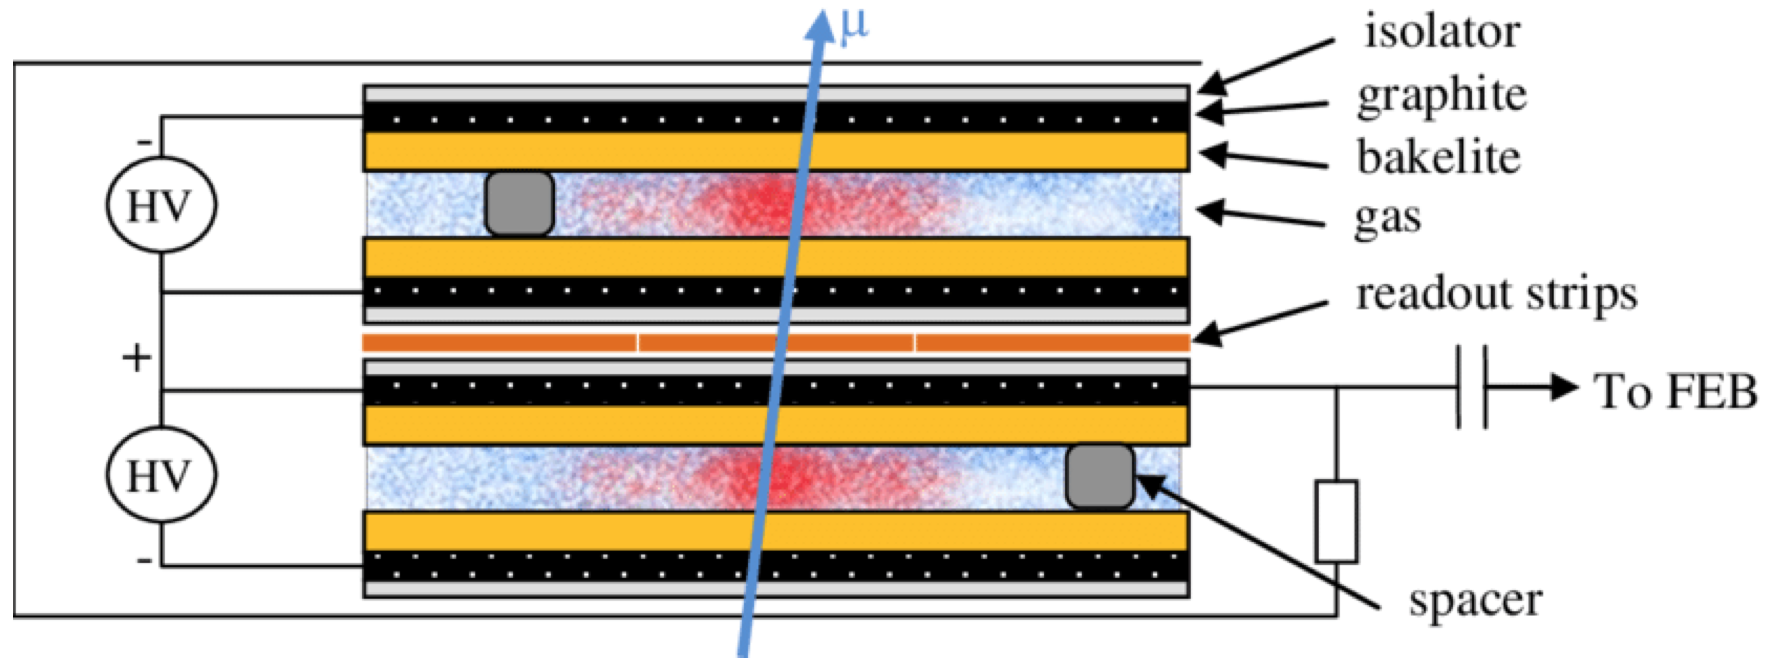
\includegraphics[width=\textwidth]{rpc.png}
	\vspace{2mm}
	\caption[Schematic view of a dual RPC detector.]{Schematic view of a dual RPC detector \cite{IanCrotty}.}
	\label{rpc}
\end{figure}

\subsection{Trigger system and storage}

The proton-proton collisions take place at the centre of the CMS detector every 25 ns, corresponding to a data of about 70 Terabytes per second. This much of data, being impossible to store with current electronics technology, mostly contains low-energy pp interactions that are not of much interest for the physics programme of the CMS Experiment; the total pp interaction cross section, that is about $10^{11} \; pb$ ($\sim98.3 \; mb$), is 5 order of magnitude larger than the frequently studied processes at the LHC \cite{ppxsec}. The task of the trigger system is to select the events that are interesting for physics analyses, reducing the acquisition rate by a factor of about $10^5$. The trigger must satisfy the technical requirements for the online data-taking and provide a high efficiency for offline data analysis \cite{Khachatryan_2017}. Specifically, with the nominal bunch crossing of the LHC, every bunch produces about 20 pp collisions resulting in about 800 M collisions per second. The corresponding data is retained and processed in pipelines, with $\sim1$ MB of memory per event making up to 70 TB per second. The trigger system decides which events to be stored in a very short time $\sim 25 \; ns$ to satisfy the LHC requirements.

The trigger systems includes two independent trigger levels. The \emph{\textbf{Level-1 Trigger}} (L1) consists of only hardware components. It reduces the the event rate from 40 MHz (corresponding to 25 ns) to a 100 kHz. The decision at L1 is made using the information from the calorimeter and the muon system. The tracker information is not used since its reconstruction time is longer than the L1 decision limit \cite{Cittolin:578006}. The L1 trigger uses the characteristics of trigger objects or trigger primitives, that are photons, leptons, jets, and $p_T$. The trigger objects are provided based on the energy deposits in the calorimeters and hit patterns in the muon chambers. The L1 trigger information from these two sub-detectors are then combined in the L1 Global Trigger (L1 GT) which takes the decision of whether to pass or reject the event.

The events that pass the L1 GT is sent to the \emph{\textbf{High Level Trigger}}, a software-based system containing multi-core computers. The task of the HLT is to reduce the event rate to be able to store the data in disks. It reduces the event rate from 100 kHz to about 1 kHz. The events that pass the requirements of at least one of the HLT trigger paths, is written permanently on disk by the \emph{\textbf{Data Acquisition System}} (DAQ) and sent to CERN Tier 0 (T0) storage system. The \emph{\textbf{Data Quality Monitoring}} (DQM) observes the recorded data and labels it in terms of quality. Finally, the collision data becomes certified and is stored as data-sets for further physics analyses.

The data that pass the trigger systems makes up to 70 PB of data every year of LHC operation, and in order to satisfy the demanding storage need, a globally distributed storage system called \emph{\textbf{World LHC Computing Grid}} (WLCG) is established in 1990s \cite{Bayatyan:838359}. The WLCG consists of the computing resources of over 170 sites in 42 countries with a total of about 900 000 processor cores and 1 Exabyte of storage. This tremendous distributed computing infrastructure grants more than 12 000 physicist around the world the access to the resources nearly the real-time. Specifically, at the end of the Run II, the transfer rates exceeded 60 GB/s globally with over 2 million tasks per day.

The WLCG consists four layers called Tiers, namely T0-1-2-3 and each tier includes several computing sites with particular tasks. Tier 0 is the CERN Data Centre and the complete set of raw data passes this facility. The first reconstruction is also made at T0 producing Primary Datasets with specific data formats; Reconstructed (RECO) and Analysis Object Data (AOD). At Run II, the RECO datasets had 4 MB of disk usage per event which was too much for the disk capabilities. Furthermore, the RECO datasets contain mostly unnecessary information for the majority of the analyses; only a few of them need all the silicon tracker hits or ECAL clusters etc. Hence the RECO datasets are not stored unless for debugging purposes. Instead, the analysis objects are chosen among RECO datasets and stored in AOD format. The AOD datasets usually contains 500 kB per event, which could still fill large storage. Another skimmed dataset is thus created to be widely used by the physics analyses at Run II, called MiniAOD. This data format reduces the precision of measurements to an acceptable level and does not include the track hits and the $p_T$ tracks that are too small. MiniAOD datasets occupy about 50 kB per event and are used by the 95 \% of physics analyses. The remaining 5 \% uses either AOD samples or further skimmed datasets called NanoAOD. The NanoAOD is the last chain in the process containing a ROOT flat ntuple where mostly the tracks are not included.

The Tier 0 distributes the raw and the RECO datasets to Tier 1 sites via the LHC Optical Private Network that consists of optical-fibre links operating at 10 Gbps, and reprocesses data outside the LHC runs. Tier 1, with 13 computing sites, stores the LHC data. It allows continuous access for the Grid as well reprocessing and storing the output. Tier 1 distributes data to Tier 2 sites, also stores a part of the simulated data coming from T2s. Tier 2s, with more than 150 sites, are typically the universities and institutes where a proportion of the LHC data is stored and some computing power is provided for the production and reconstruction of simulated event samples. Finally, Tier 3 is formed by the individual researchers accessing to Grid from local computing resources with no formal engagement with WLGC.

\section{The HL-LHC Programme and the Phase II Upgrade of the CMS Detector}

The inaugural schedule of the LHC programme, detailed in \autoref{HLLHCplan}, is aimed to reach its final design expectations, so called the \emph{\textbf{High-Luminosity LHC}}, at the end of the 2020s. The integrated luminosity delivered is expected to be 3000 - 4000 $fb^{-1}$ for pp collisions and, PbPb and pPb collisions with integrated luminosities of 13 $nb^{-1}$ and 50 $nb^{-1}$, respectively, in 2030s and onwards. If the HL-LHC upgrades were not to be realised, the total integrated luminosity for another 10 years of operation would be around 1000 $fb^{-1}$ \cite{Aleksan:1628377}. In any case, the current LHC inner triplets will have to be replaced after an integrated luminosity of 400 $fb^{-1}$.

The average pile-up will reach 200 per bunch crossing while providing a centre-of-mass energy of 14 TeV, which will surely impose a demanding environment for the detectors around the LHC ring. Especially, after the discovery of the SM Higgs boson, the case study for an HL-LHC is easier to define and quantify \cite{cmsloi}. The SM expects the discovery of all final states of the Higgs boson given a high integrated luminosity, for example the decays $H\rightarrow\mu^+\mu^-$ and $H\rightarrow Z\gamma$ have the need of an integrated luminosity on the order of 3000 $fb^{-1}$, which supports the HL-LHC programme.

The excess amount of data will also provide higher-precision measurements of the Higgs couplings, for instance in the $HH\rightarrow\tau\tau bb$ and $HH\rightarrow\gamma\gamma bb$ \cite{ATLAS:1502664}. In addition to the SM Higgs sensitivity, the BSM models such as supersymmetric partners of quarks and gluons with mass greater than 1.5 $TeV/c^2$ will benefit from the high amount of data. Another example is the new $Z^\prime$ bosons which would show the existence of new weak interactions with the HL-LHC programme if its mass is above 2.5 $TeV/c^2$.

In this context, the demanding conditions of the HL-LHC such as the increased luminosity and the higher pile-up, entails a major upgrade to the current \emph{\textbf{CMS detector}} in order exploit the physics potential. The pixel and strip tracker detectors will be replaced in order to increase the granularity, enhance the radiation hardness, decrease the material budget and provide extended geometrical acceptance up to $\eta = |4|$. The front-end electronics of the barrel ECAL will be upgraded to be able to access single crystal information at L1 trigger, to provide 160 MHz sampling which allows high precision timing capability for photons, and to accommodate bandwidth requirements and trigger latency. The muon system will undergo upgrades for its 3 types of gaseous detectors; new muon detectors with enhanced RPC and gas electron multiplier technologies will contribute to the redundancy of the detector, increase the pseudorapidity coverage up to $ \eta = |2.8|$ and enhance the trigger and reconstruction performance in the forward region. The endcap ECAL and HCAL will be replaced with an advanced combined sampling calorimeter which will provide higher-precision timing information and higher-segmented spatial information both in the longitudinal direction and the transverse plane. A new timing detector will be added for minimum ionising particles in both barrel and endcap regions and aimed at better reconstruction of interaction vertices. This upgrade will also help mitigate the performance derogation due to high pile-up. Finally, the complete trigger system; L1, HLT and DAQ will be upgraded substantially \cite{Contardo:2020886}.